% !TeX spellcheck = en_US
\documentclass[a4paper,11pt]{article}
\usepackage[left=2.5cm, top=2.5cm, right=2.7cm, bottom=2.4cm]{geometry}
\usepackage[utf8]{inputenc}
\usepackage[english]{babel}
\usepackage{amsfonts}
\usepackage{tipa}
\usepackage{url}
\usepackage{pgfplots}
\pgfplotsset{compat=1.12}
\usepackage{csvsimple}
\usepackage{filecontents}
\usepackage{pgfplotstable}
\usepackage{tikz, pgf, pgfplots, pgfplotstable}
\usepackage{transparent}
\usepackage{subfig}
%\usepackage{showframe}
\usetikzlibrary{patterns}
%\usepgfplotslibrary{groupplots} % LATEX and plain TEX
%\usepgfplotslibrary{colorbrewer}
\usetikzlibrary{plotmarks}
\usepackage{float}
\usepackage{booktabs}
\usepackage{listings} %For code in appendix
\lstset{%
    basicstyle=\ttfamily,
    commentstyle = \color{gray},
    frame=single,
    numbers=left,
    language=C,
    breaklines=true,
    columns=fullflexible,
    tabsize = 4,
    breakindent=0pt}

\usepackage{fancyvrb}

\usepackage{datatool}
\DTLsetseparator{,}

\DTLloaddb{tal}{reading-list/plo-word-list.csv}
\DTLloaddb{tal2}{reading-list/fr-word-list.csv}

\DTLloaddb{gtal}{reading-list/plo-gl-word-list.csv}
\DTLloaddb{gtal2}{reading-list/fr-gl-word-list.csv}
\usepackage{multicol}

\usepackage{pgfmath}

% code for generating a random permutation
\newcounter{randomListLength}%   current length of our random list
\newcounter{randomListPosition}% current list index
\newcounter{newRandomListElementPosition}% position to insert new element
% insert #1 into the next position of \newRandomList unless the position
% index \randomListPosition is equal to \newRandomListElementPosition in
% which case the \newRandomListElement is added first
\newcommand\randomlyInsertElement[1]{%
    \stepcounter{randomListPosition}%
    \ifnum\value{randomListPosition}=\value{newRandomListElementPosition}%
    \listxadd\newRandomList{\newRandomListElement}%
    \fi%
    \listxadd\newRandomList{#1}%
}
% \randomlyInsertInList{list name}{new list length}{new element}
\newcommand\randomlyInsertInList[3]{%
    \pgfmathparse{random(1,#2)}%
    \setcounter{newRandomListElementPosition}{\pgfmathresult}%
    \ifnum\value{newRandomListElementPosition}=#2\relax%
    \listcsxadd{#1}{#3}%
    \else%
    \def\newRandomList{}% start with an empty list
    \def\newRandomListElement{#3}% and the element that we need to add
    \setcounter{randomListPosition}{0}% starting from position 0
    \xdef\currentList{\csuse{#1}}
    \forlistloop\randomlyInsertElement\currentList%
    \csxdef{#1}{\newRandomList}%
    \fi%
}

% define some pgfkeys to allow key-value arguments
\pgfkeys{/randomList/.is family, /randomList,
    environment/.code = {\global\letcs\beginRandomListEnvironment{#1}
        \global\letcs\endRandomListEnvironment{end#1}
    },
    enumerate/.style = {environment=enumerate},
    itemize/.style = {environment=itemize},
    description/.style = {environment=description},
    seed/.code = {\pgfmathsetseed{#1}}
}
\pgfkeys{/randomList, enumerate}% enumerate is the default

% finally, the code to construct the randomly permuted list
\makeatletter
\newcounter{randomListCounter}% for constructing \randomListItem@<k>'s

% \useRandomItem{k} prints item number k
\newcommand\useRandomItem[1]{\csname randomListItem@#1\endcsname}

% \setRandomItem{k} saves item number k for future use
% and builds a random permutation at the same time
\def\setRandomItem#1\par{\stepcounter{randomListCounter}%
    \expandafter\protected@xdef\csname randomListItem@\therandomListCounter\endcsname{\noexpand\item#1}%
    \randomlyInsertInList{randomlyOrderedList}{\therandomListCounter}{\therandomListCounter}%
}%
\let\realitem=\item
\makeatother
\newenvironment{randomList}[1][]{% optional argument -> pgfkeys
    \pgfkeys{/randomList, #1}% process optional arguments
    \setcounter{randomListLength}{0}% initialise length of random list
    \def\randomlyOrderedList{}% initialise the random list of items
    % Nthing is printed in the main environment. Instead, \item is
    % used to slurp the "contents" of the item into randomListItem@<counter>
    \let\item\setRandomItem%      
}
{% now construct the list environment by looping over the randomly ordered list
    \let\item\realitem
    \setcounter{randomListCounter}{0}
    \beginRandomListEnvironment\relax
    \forlistloop\useRandomItem\randomlyOrderedList
    \endRandomListEnvironment
}

% test compatibility with enumitem
\usepackage{enumitem}
\newlist{Testlist}{enumerate}{1} %
\setlist[Testlist]{label*=\alph*.}
%\setlist{nosep}\parindent=10pt% for more compact output
%\pgfplotsset{cycle list/Dark2}



%% defining the new dimensions
%\newlength{\starsize}
%\newlength{\starspread}
%% declaring the keys in tikz
%\tikzset{starsize/.code={\setlength{\starsize}{#1}},
%    starspread/.code={\setlength{\starspread}{#1}}}
%% setting the default values
%\tikzset{starsize=1mm,
%    starspread=3mm}
%% declaring the pattern
%\pgfdeclarepatternformonly[\starspread,\starsize]% variables
%{custom fivepointed stars}% name
%{\pgfpointorigin}% lower left corner
%{\pgfqpoint{\starspread}{\starspread}}% upper right corner
%{\pgfqpoint{\starspread}{\starspread}}% tilesize
%{% shape description
%    \pgftransformshift{\pgfqpoint{\starsize}{\starsize}}
%    \pgfpathmoveto{\pgfqpointpolar{18}{\starsize}}
%    \pgfpathlineto{\pgfqpointpolar{162}{\starsize}}
%    \pgfpathlineto{\pgfqpointpolar{306}{\starsize}}
%    \pgfpathlineto{\pgfqpointpolar{90}{\starsize}}
%    \pgfpathlineto{\pgfqpointpolar{234}{\starsize}}
%    \pgfpathclose%
%    \pgfusepath{fill}
%}
\usepackage{amsmath,lipsum}
\newcommand{\mypm}{\mathbin{\smash{%
            \raisebox{0.35ex}{%
                $\underset{\raisebox{0.5ex}{$\smash -$}}{\smash+}$%
            }%
        }%
    }%
}

\usetikzlibrary{pgfplots.statistics}        % to draw `boxplot's
\pgfplotstabletranspose\mytable{trial.dat}  % transpose the data table

\pgfdeclareplotmark{training}{\pgfuseplotmark{*}}
\pgfdeclareplotmark{validation}{\pgfuseplotmark{square}}

\definecolor{n1}{RGB}{230,25,75}
\definecolor{n2}{RGB}{60,180,75}
\definecolor{n3}{RGB}{255,255,25}
\definecolor{n4}{RGB}{0,130,200}
\definecolor{n5}{RGB}{245,130,48}
\definecolor{n6}{RGB}{145,30,180}
\definecolor{n7}{RGB}{70,240,240}
\definecolor{n8}{RGB}{240,50,230}
\definecolor{n9}{RGB}{210,245,60}
\definecolor{n10}{RGB}{250,190,190}
\definecolor{n11}{RGB}{0,128,128}
\definecolor{n12}{RGB}{230,190,255}
\definecolor{n13}{RGB}{170,110,40}
\definecolor{n14}{RGB}{255,250,200}
\definecolor{n15}{RGB}{128,0,0}
\definecolor{n16}{RGB}{170,255,195}
\definecolor{n17}{RGB}{128,128,0}
\definecolor{n18}{RGB}{255,215,180}
\definecolor{n19}{RGB}{0,0,128}
\definecolor{n20}{RGB}{128,128,128}

\usepgfplotslibrary{groupplots} % LATEX and plain TEX
\begin{filecontents}{data.dat}
    QoI model surrogate type outname QoI_group error_scaled
    A -1 -1.01224658575 training Q1 1 0.014956929466                      % Color 1, mark style 1 (until "type"="validation")
    A -0.977952092966 -0.984618496392 training Q1 1 0.014956929466        % Color 1
    B 0.53568190987 0.521776331357 training Q2 1 0.0158105026132          % Color 2
    B 0.798208448928 0.789090773894 training Q3 1 0.044540998773          % Color 3
    C 0.378407928561 0.326243792219 training Q4 1 0.0274695358287         % Color 4
    C 0.355049936935 0.33464474407 training Q4 1 0.0274695358287          % Color 4
    D 0.762183505103 0.681415197111 validation Q3 1 0.044540998773        % Color 3, mark style 2
    D 0.822636091166 1.02086372811 validation Q3 1 0.044540998773         % Color 3, mark style 2
\end{filecontents}

\pgfmathdeclarefunction{fpumod}{2}{%
    \pgfmathfloatdivide{#1}{#2}%
    \pgfmathfloatint{\pgfmathresult}%
    \pgfmathfloatmultiply{\pgfmathresult}{#2}%
    \pgfmathfloatsubtract{#1}{\pgfmathresult}%
    % replaced `0' by `5' to make it work for this problem
    \pgfmathfloatifapproxequalrel{\pgfmathresult}{#2}{\def\pgfmathresult{4.5}}{}%
}

\pgfplotscreateplotcyclelist{full}{%
    blue,every mark/.append style={fill=blue!80!black},mark=*,solid\\%
    red,every mark/.append style={fill=red!80!black,solid},mark=square*\\%
    n11,every mark/.append style={fill=n11!80!black,solid,thin},mark=diamond*\\%
%    black,mark=triangle*,every mark/.append style={solid,fill=gray},dashdotted\\%
%    blue,every mark/.append style={fill=blue!80!black},mark=o,solid\\%
%    red,every mark/.append style={fill=red!80!black,solid},mark=square,dashed\\%
%    brown!60!black,every mark/.append style={fill=brown!80!black,solid,thin},mark=diamond,dotted,thick\\%
%    black,mark=triangle,every mark/.append style={solid},dashdotted\\%
}


\pgfplotsset{
    discard if not/.style 2 args={
        x filter/.code={
            \edef\tempa{\thisrow{#1}}
            \edef\tempb{#2}
            \ifx\tempa\tempb
            \else
            \def\pgfmathresult{inf}
            \fi
        }
    }
}

\newcommand{\plotphoneme}[3]{
\addplot [
color=#3,
discard if not={phoneme}{#2},
scatter,
scatter src=explicit symbolic,
mark=text,
only marks,
scatter/@pre marker code/.code={\pgfplotsset{text mark=\textipa{\pgfplotspointmeta}}},
scatter/@post marker code/.code={}
] table [x=F2, 
y=F1, 
col sep=comma,
meta=phoneme] {#1};
}

\newcommand{\plotallphonemes}[1]{
\plotphoneme{#1}{a}{n1}
\plotphoneme{#1}{e}{n2}
\plotphoneme{#1}{o}{n10}
\plotphoneme{#1}{O}{n4}
\plotphoneme{#1}{u}{n5}
\plotphoneme{#1}{U}{n6}
\plotphoneme{#1}{E}{n7}
\plotphoneme{#1}{I}{n8}
\plotphoneme{#1}{5}{n9}
\plotphoneme{#1}{\~a}{n11}
\plotphoneme{#1}{\~e}{n12}
\plotphoneme{#1}{\~i}{n15}
\plotphoneme{#1}{ZI}{n8}
\plotphoneme{#1}{zI}{n8}
\plotphoneme{#1}{\~o}{n10}
\plotphoneme{#1}{i}{n15}
}


\begin{document}
	
	\title{An acoustic study on the vowels of three Galician-Portuguese varieties}
	\author{Pedro González Bascoy\\
		\texttt{st168913@stud.uni-stuttgart.de}\\
		\\Institut für Maschinelle Sprachverarbeitung}
	
	\maketitle
	
    
  \begin{abstract}
      This work analyzes the acoustic dissimilarities between Galician, European Portuguese and Brazilian Portuguese: three different varieties of the Galician-Portuguese language. The study focuses on vowel inventories, which are captured thanks to the recordings carried out by  three native speakers. Vowels are manually tagged and then measured in terms of lengths and formants frequencies using the tool \texttt{praat} in an automatic fashion. The formant and duration analysis suggests that Galician and Brazilian Portuguese might be acoustically closer to each other than to European Portuguese, even though they themselves have never been into direct contact.
  \end{abstract}
    
    \section{Introduction}
    
    Languages are dynamic entities, constantly evolving in time. Modern languages are the product of centuries of language evolution on ancient, dead languages. Normally, languages are organized following a hierarchical structure that intrinsically shows their relationships with other surrounding languages. The Germanic and Romance languages constitute some examples of language families within Europe, which throughout the last twenty centuries evolved into a number of ``dialects'' that are currently spoken all across northern and southern west Europe. The evolution of languages, however, has always responded to political and social affairs more than actual chance. In this sense, for instance, the Latin dialects (``Vulgar Latin'') spoken throughout the area of the Roman Empire led to the development of the languages in southern Europe (such as Spanish, Italian and French among others) when the identities and regions of the old Empire coalesced into different countries.\\
    
    Portuguese and Galician currently constitute  the leafs of the Ibero-Romance branch of the Western Romance Languages. Portuguese is the official language of Portugal and Brazil, with some  speaker minorities in former Portuguese colonies in southern Africa. Galician in contrast, is a co-official language (along with Spanish) in the autonomous community of Galicia, in north west Spain. The similarities between Galician and Portuguese languages are not arbitrary, as both are spoken in areas that share country borders in the west of the Iberian peninsula. At the same time, both are varieties of the same common ancestor called -- depending on the source -- Galician-Portuguese (the most used term), Old Portuguese or Medieval Galician, which developed as a distinctive Latin dialect in the 8th century. It was spoken throughout the middle ages in an area including the current territory of Galicia and the north of Portugal. In the 16th century, while Galician-Portuguese was being introduced into the American colonies (current territory of Brazil), it started to diverge into a number of separated dialects motivated by political affairs: the territories where the language was spoken were divided in the 13th century into the kingdoms of León and Portugal. León acquired  control of the Galician territory and since that time on, the future of the northern and southern Galician-Portuguese dialects was decided for good. The southern dialect could thrive as the official language of the kingdom of Portugal (established by King Denis) whereas the northern dialect gradually suffered the oppression of the Castilian (Spanish) language, surviving the following centuries in a situation of diglossia. Nowadays, both languages are reported to be mutually intelligible and to have a high percentage of cognates, i.e. words that have a common ancestor. Moreover, there is still a language continuum from the Cantabrian See (northern Spain) all the way down to the Algarve (southern Portugal), specially from the phonological point of view. The phonological features of both languages are clearly distinct, having Galician lost many characteristics of Galician-Portuguese and adopting not only some aspects of the Spanish phonology but also its orthography. Separately, the Brazilian dialect of Portuguese (BP), or as coined in \cite{escudero}, the age-, social-economic-status, and region dependent variety of the standard language; has evolved independently from European Portuguese (EP) as many other non-native American languages  (English, Spanish, French, etc) introduced in the colony era. In this sense, BP has its own distinctive set of phonemes and vocabulary, as we would expect in Latin American Spanish or in American English. \\
    
    
    In spite of Brazil not belonging to the language continuum described above, there is a generalized perception that BP is closer than EP  to the Galician phonology inside the autonomous community: Galician native speakers often find less difficulties to understand the BP than the European variant, although Galician and Portuguese are considered nowadays distinctive different languages. This general feeling has not been described or characterized before in a formal study, thus the purpose of this novel work is to investigate the acoustic characteristics of Galician, EP and BP and describe whether this phenomenon can be determined by empirical data. Nevertheless, the phonological characteristics of the languages at stake have been independently studied before. A comprehensive study of the Galician phonology can be found in \cite{blancoo} (in Galician) and the Portuguese variants have been thoroughly described in many other works \cite{camara,delgado,matos} (in Portuguese). As the amount of work needed to carry out experiments for all three languages concerning all phonological aspects is beyond the purpose of this report, the experiments will only focus on vowels for a number of reasons: (1) the vowel inventory is reduced as compared to the consonant set, (2) all three languages partially share  vowel inventory \cite{moraes,barroso} and (3) there are evidences that the behavior of vowel reduction in Galician is significantly less than the EP and comparable to BP \cite{figueiroa,regueira}. As stated above, EP and BP are said to have an internal symmetric vowel inventory consisting of three unrounded front vowels (\textipa{i, e, E}) and three rounded vowels (\textipa{u, o, O}) that can be identified in pairs as follows: two high vowels (i, u), two higher-mid vowels (e, o) and finally two lower-mid vowels (\textipa{E, O}). Following the phonetic description stated in \cite{blancoo}, the Galician language also fulfills this inventory. Similarly, all three languages have been reported to have no phonological length distinctions in vowels \cite{mateus}, but in \cite{escudero} is shown that Portuguese speakers seem to have turned vowel duration into a clue for vowel identity and that in general BP vowels are longer that EP ones. This could be connected with the fact that, like English, all three languages are time stressed, so vowels [\textipa{a, o, e}] in non stressed syllables tend to be reduced to [\textipa{5, U, I}]. However, the work in \cite{dubert} shows that the reduction made in the Galician is much relaxed, to the point that according to Dubert's transcriptions, the word ``noite'' (Galician and Portuguese for ``night'') is transcribed as noit\textipa{[\textraising{e}]} instead of \textipa{noit[I]}. Following the same direction, \cite{regueira} also notices that the reduced vowel, if present at all, is normally longer than the BP and EP counterparts and also lower ( however, ``noite'' could be transcribed as \textipa{noit[1]} in EP). \\
    
    The present work aims to characterize the common symmetrical vowels (\textipa{i, e, E, a, u, o, O}) and its realizations in non-stressed syllables of two varieties  of the Galician-Portuguese language, namely Galician and Portuguese (from now on, dialects). To accomplish so, the work will also focus on two varieties of Portuguese: EP and BP; and will provide measurements of vowels between unvoiced consonants and their formant values. The data collected will be used to study the validity of the undocumented phenomenon related to the degree of understanding between Galician-Portuguese varieties, paying special attention in the Galician-BP and Galician-EP directions.
    
    %TODO: describe the following sections (as if it was a paper).
    
    \section{Method}
    In this section the participants, the data collection methodology and the data treatment are introduced.
    
    \subsection{Participants}
    
    As the study is targeting two varieties of Galician-Portuguese and two varieties of Portuguese, native speakers of each dialect are required. The ideal scenario would be such that at least ten speakers of each language and gender would take part in the recording sessions. Unfortunately, the author of this work does not have the contacts, materials, time and resources to carry out such comprehensive data collection. In this regard, the number of speakers that would be needed would rise up to sixty: twenty speakers for each dialect, being 50 \% women and 50 \% men. In the actual study, however, only three speakers took part in the recording sessions. Since the number of speakers is reduced from the best-case situation, it is important that the selection of informants is done by minimizing the individual characteristics among them. In this concern, the Galician participant is the author of this work itself. This is far from being optimal, but Galician native speakers are not as easy to find as Portuguese native speakers (specially  taking into consideration that this study is being carried out in the south of Germany) due to the reduced number of Galician population ($2,699,499$ inhabitants \cite{ige} at the time of writing this report) that can actually fluently speak the language (according to \cite{persoas}, 27.74 \% of the Galician population, i.e. only $748,899$ inhabitants,  have got Galician as their first mothertongue and is currently the language they know best). By these means, the author of the document is a good candidate: a 24 year old male from Santiago de Compostela who has been in touch with Galician throughout his childhood and who nowadays has a reasonable level of competence. As far as the Portuguese informants are concerned, on the one hand the EP participant is a 25 year old male university student born and raised in the small coastal town of Portim\~ao, in southern Portugal. In terms of the language continuum mentioned in the introduction, Portim\~ao and Santiago de Compostela represent an extreme scenario since both are as distal  as they can physically be. On the other hand, the 26 year old male BP speaker comes from the city of Rio de Janeiro, and he is currently studying at University of Hohenheim. %TODO add some description of how the portuguese in that area is like.
     Finally, it is worth noting that all participants were males whose mean age was 25 and none of them had ear diseases at the time of carrying out the experiments.
     
     \subsection{Collection of experimental data}
     
     The recordings were made in two different locations and equipment due to budget constraints. In particular, the ones made by the Galician and BP informants were carried out in the quiet room available in the Institut für Maschinelle Sprachverarbeitung (IMS) at University of Stuttgart. The set-up consisted in a console Yamaha CL1 recorder and a Neumann type U87 P48 condenser microphone with a sample rate of 41.1 kHz (high enough for characterizing vowels) and a high quality 24-bit quantization. On the contrary, the EP recordings were made in situ at the residence of the informant, in Lisbon. His setup consisted of a Xiaomi MI smartphone equipped with a built-in microphone, the same 41.1 kHz sampling rate used in the phonetics lab and 16-bit quantization.\\
     
     The reading lists created aimed to collect (to some extent) the symmetric vowels present in the dialects (\textipa{i, e, E, a, u, o, O}), and have been carefully designed to include multiple samples of the vowels that appear in unstressed syllables at the end of words. The grammatical rules of Galician and Portuguese mostly limit the sounds in unstressed vowels to be realized as /\textipa{5, U, I}/\cite{BORGES2000} in BP,   /\textipa{5, U, 1}/ \cite{mateus2000phonology} in EP and  /\textipa{\textraising{a}, \textraising{o} or \textraising{e}}/ or /\textipa{5, U, I}/ \cite{figueiroa} in Galician depending on the accounted source, as stated in the introduction. This phenomenon is mainly produced because most of the word endings finish with either \textipa{a, o, e},  which represent the phones described above, respectively. Words ending in unstressed vowels i, u are unusual and therefore they are not included into this study. Additionally, following the recommendations given in the lectures, nonce words were avoided as they are more difficult to pronounce in a natural fashion. It is worth noting that the difficulty of creating a common reading list in two different languages, in spite of being one akin to the other, is very high. In this sense, words appearing in the reading list were chosen independently of the actual meaning in each language, e.g. the word ``fixe'' stands for ``cool'' in Portuguese while in Galician is the past tense of the verb ``to do'', and independently of the spelling rules of each language, e.g. the word pineapple is spelled ``pinha'' in Portuguese and ``piña'' in Galician, even though ``nh'' and ``ñ'' represent both the phoneme /\textipa{\textltailn}/\footnote{The digraph ``nh'' in Galician stands for the phoneme /\textipa{N}/.}.   To avoid further complexity on the reading lists beyond the actual differences in the dialects, only bisyllabic words in the form CVCV (``C'' stands for consonant and ``V'' for vowel) were included. Consonants were preferred to be plosives such as /p,~t,~k/ or voiceless fricatives e.g. /f,~s,~\textipa{S},~\textipa{T}/, as avoiding the vocal fold vibration will automatically isolate the vowels in the spectrogram, easing their identification. Furthermore, all the words in the reading lists are stressed in the first syllable, producing reductions only at the last ones. As stated above, the reading lists contain words for all the vowels aimed to be studied, which can be divided into the following categories: (1) twenty words ending in ``o'' for stuying the realization of phonemes /\textipa{U}/ or /\textipa{\textraising{o}}/ such as ``lixo'' (trash), (2) twenty words ending in ``a'' for the realization of the phoneme /\textipa{5}/ or /\textipa{\textraising{a}}/ e.g. ``fusa'' (fuse) and (3) twenty words ending in ``e'' for studying the realization of the phoneme /\textipa{I}/,  /\textipa{1}/ or /\textipa{\textraising{e}}/, for instance ``sete'' (seven). At the same time, each set of twenty words is subdivided into two sets of ten words so that the second consonant of the word (CV\textbf{C}V) is either a fricative or a plosive (e.g. ``fofo'' (fat) and ``peto'' (pocket)). This is done because the  type of consonant preceeding the unstressed vowel could affect the length and its characteristics, and it is aim of this work to investigate that as well. Finally, the same set of sixty words were added to a separated reading list but pluralized (the inflection is done by attaching -s to the end of the words) also to study the degree of influence fricatives have in the coda of unstressed syllables.\\
     
     Words were presented to the participants not isolated but embedded into the phrase ``\texttt{DIGA <TARGET\string_WORD> DE NOVO.}'' which is Galician and Portuguese for ``\texttt{SAY <TARGET\string_WORD> AGAIN.}'' and shuffled, so not all the endings were all in a row. In the case that during the recording any participant misread a word or a sentence, informants were asked to repeat them afterwards. Each participant produced 40 tokens of each vowel embedded in two different consonants contexts (frivative vs. plosive second consonant + nothing or -s ending), therefore a total of $40\times 3\times 3 = 360$ tokens aimed to be studied.
     
     \subsection{Data analysis}
     
     The acquired waveforms were tagged and processed using the \texttt{praat} \cite{Boersma2009} software, which is currently one of the most powerful free-licensed tools for phonetic analysis in computers. The next lines detail how the tagging process and the vowel feature extraction was made.
     
     \subsubsection{Data tagging}
     
     The recording sessions generated two different wavefiles for each language, one with the words of the regular reading list and another one with the pluralized words (both can be found in Appendix \ref{sec:reading-lists}), as stated in the section above. For each one of these files, manual tagging of vowels (C\textbf{V}C\textbf{V}) in words was made using the annotation tool \texttt{TextGrid} that is built-in \texttt{praat}. It was carried out attending to (1) stability of the vowel throughout time, (2) explicity phonation seen in the bottom side of the spectrogram, and (3) the phonetic dictionary of Portuguese \cite{dicionario} to assess the identification of phonemes (only in stressed syllables).
     
% TODO: \usepackage{graphicx} required
\begin{figure}[htbp]
    \centering
    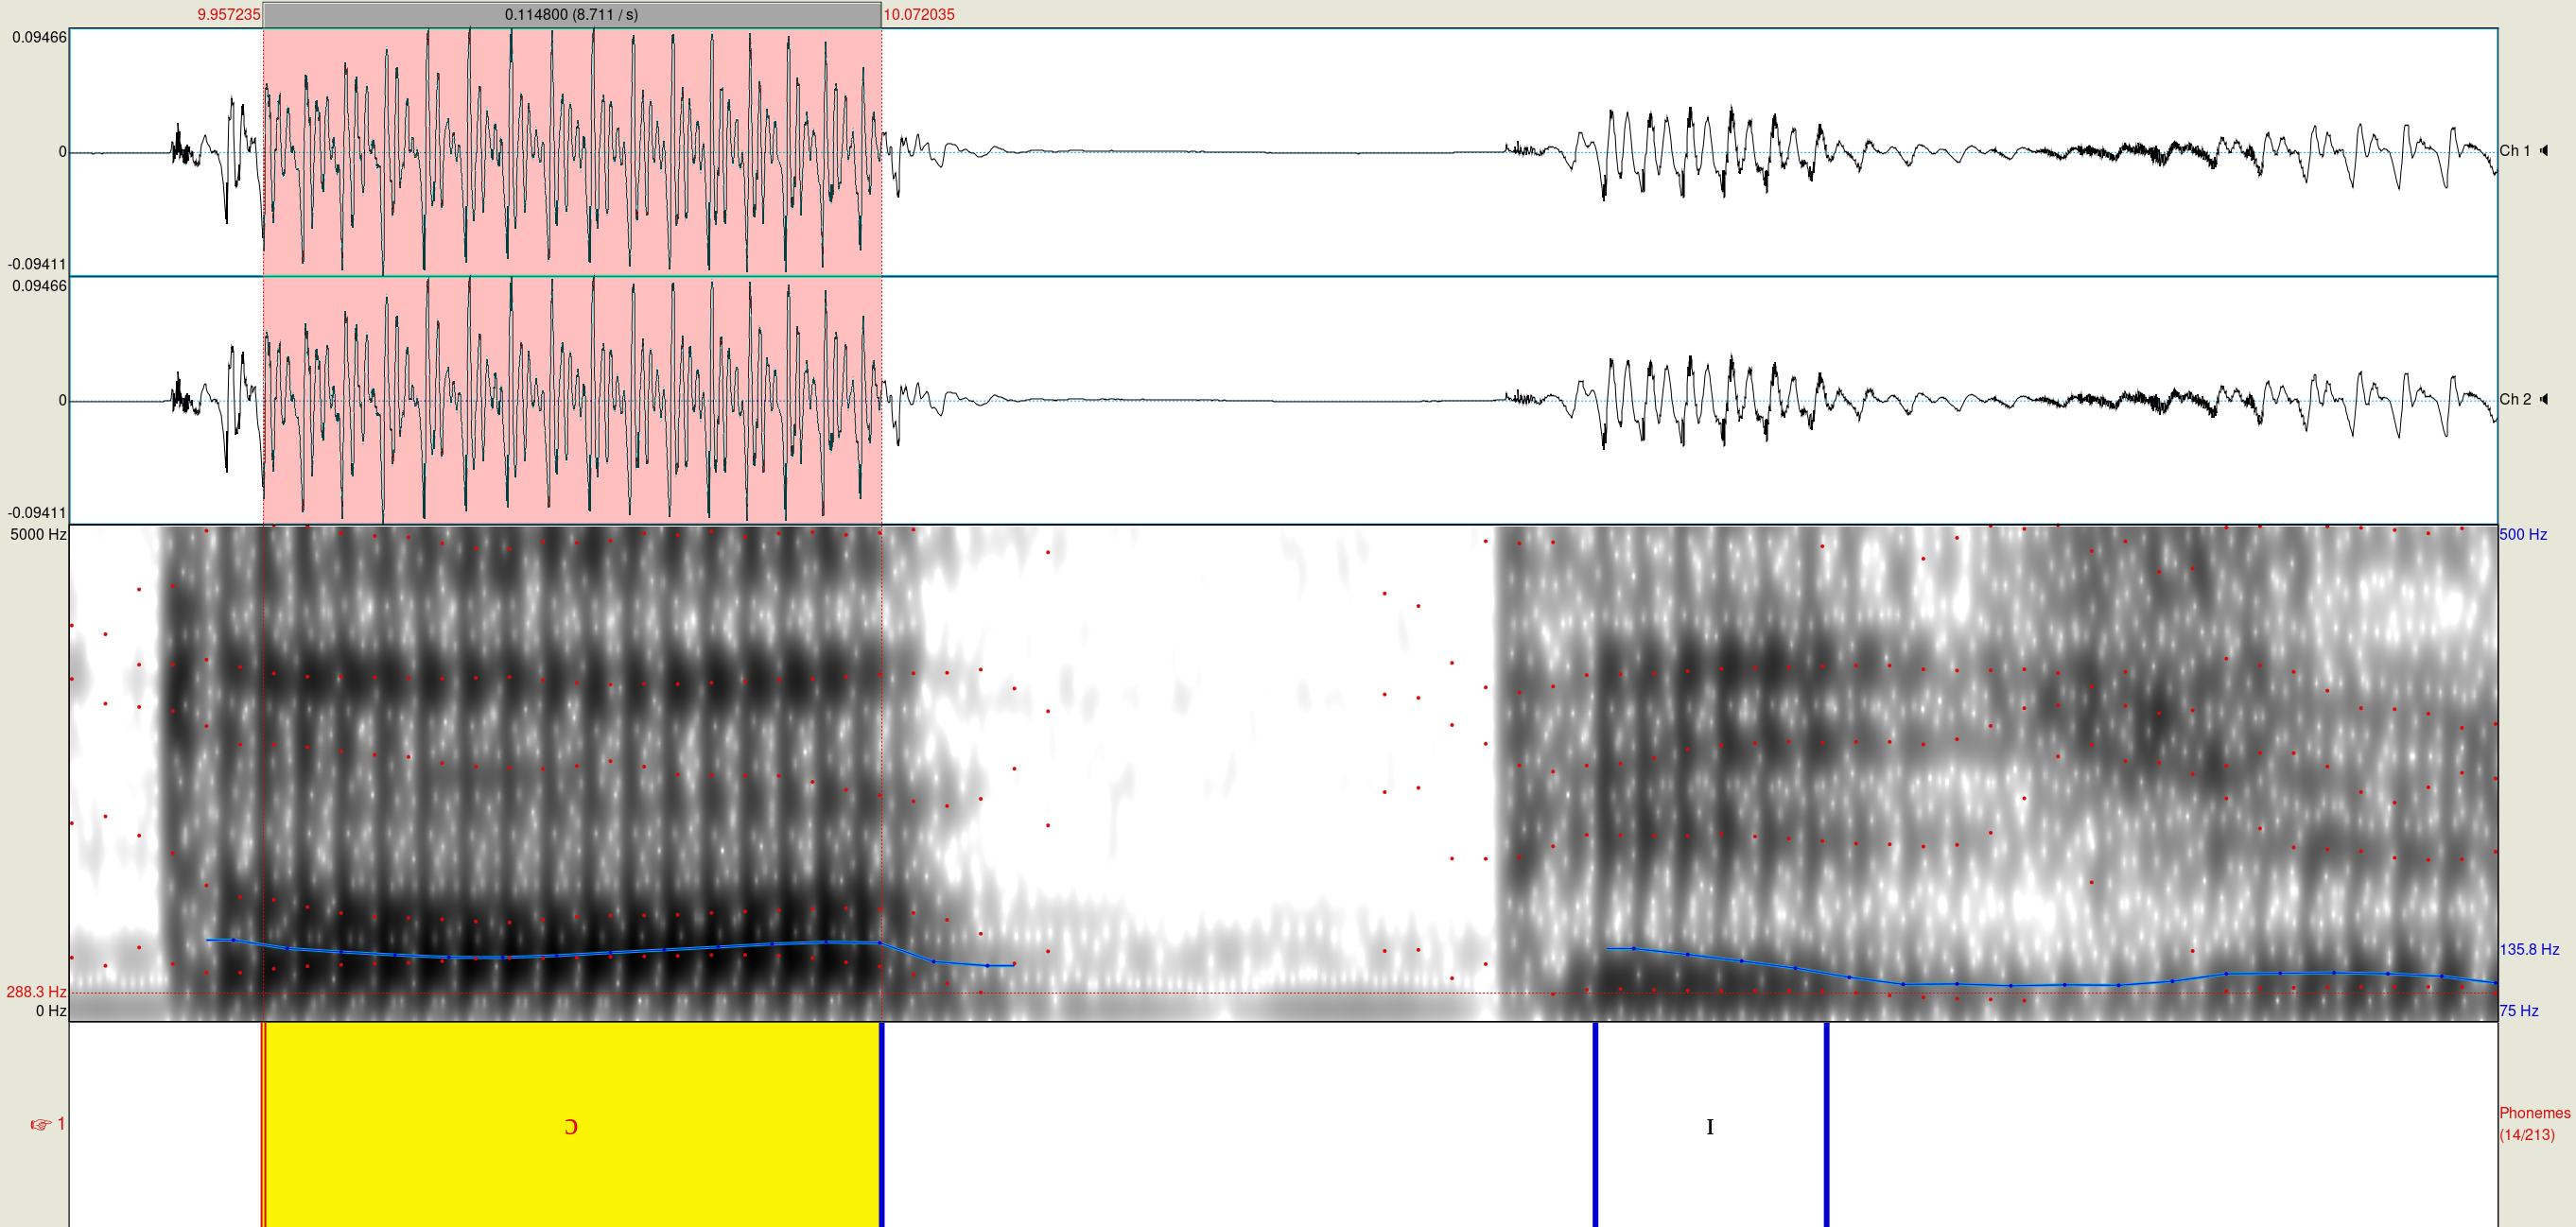
\includegraphics[width=0.6\linewidth]{figs/tope-bp}
    \caption{The phoneme /\textipa{O}/ tagged in the word ``tope'' /\textipa{tOpI}/ (summit) as spoken by the Brazilian informant.}
    \label{fig:tope-bp}
\end{figure}

The stability of the vowel is vital to correctly measure its first and second formants. As seen in Figure \ref{fig:tope-bp}, the tagged phone /\textipa{O}/ is not embracing the whole phonation but only the most stable part. The same can be seen for the phone /\textipa{I}/. In this case the initial and final part of the vowel are discarded as phonation is not clearly seen in the bottom of the broad-band spectrogram. On the other hand, in case that the reduction is such that a vowel can not be clearly distinguish or does not appear at all, it would not be tagged and thus not included in the processing described below. This scenario is specially common for EP, because many reductions end up with a not realization of a vowel (Figure \ref{fig:tope-ep}). This behavior will be further discussed in the results section. 
% TODO: \usepackage{graphicx} required
\begin{figure}[htbp]
    \centering
    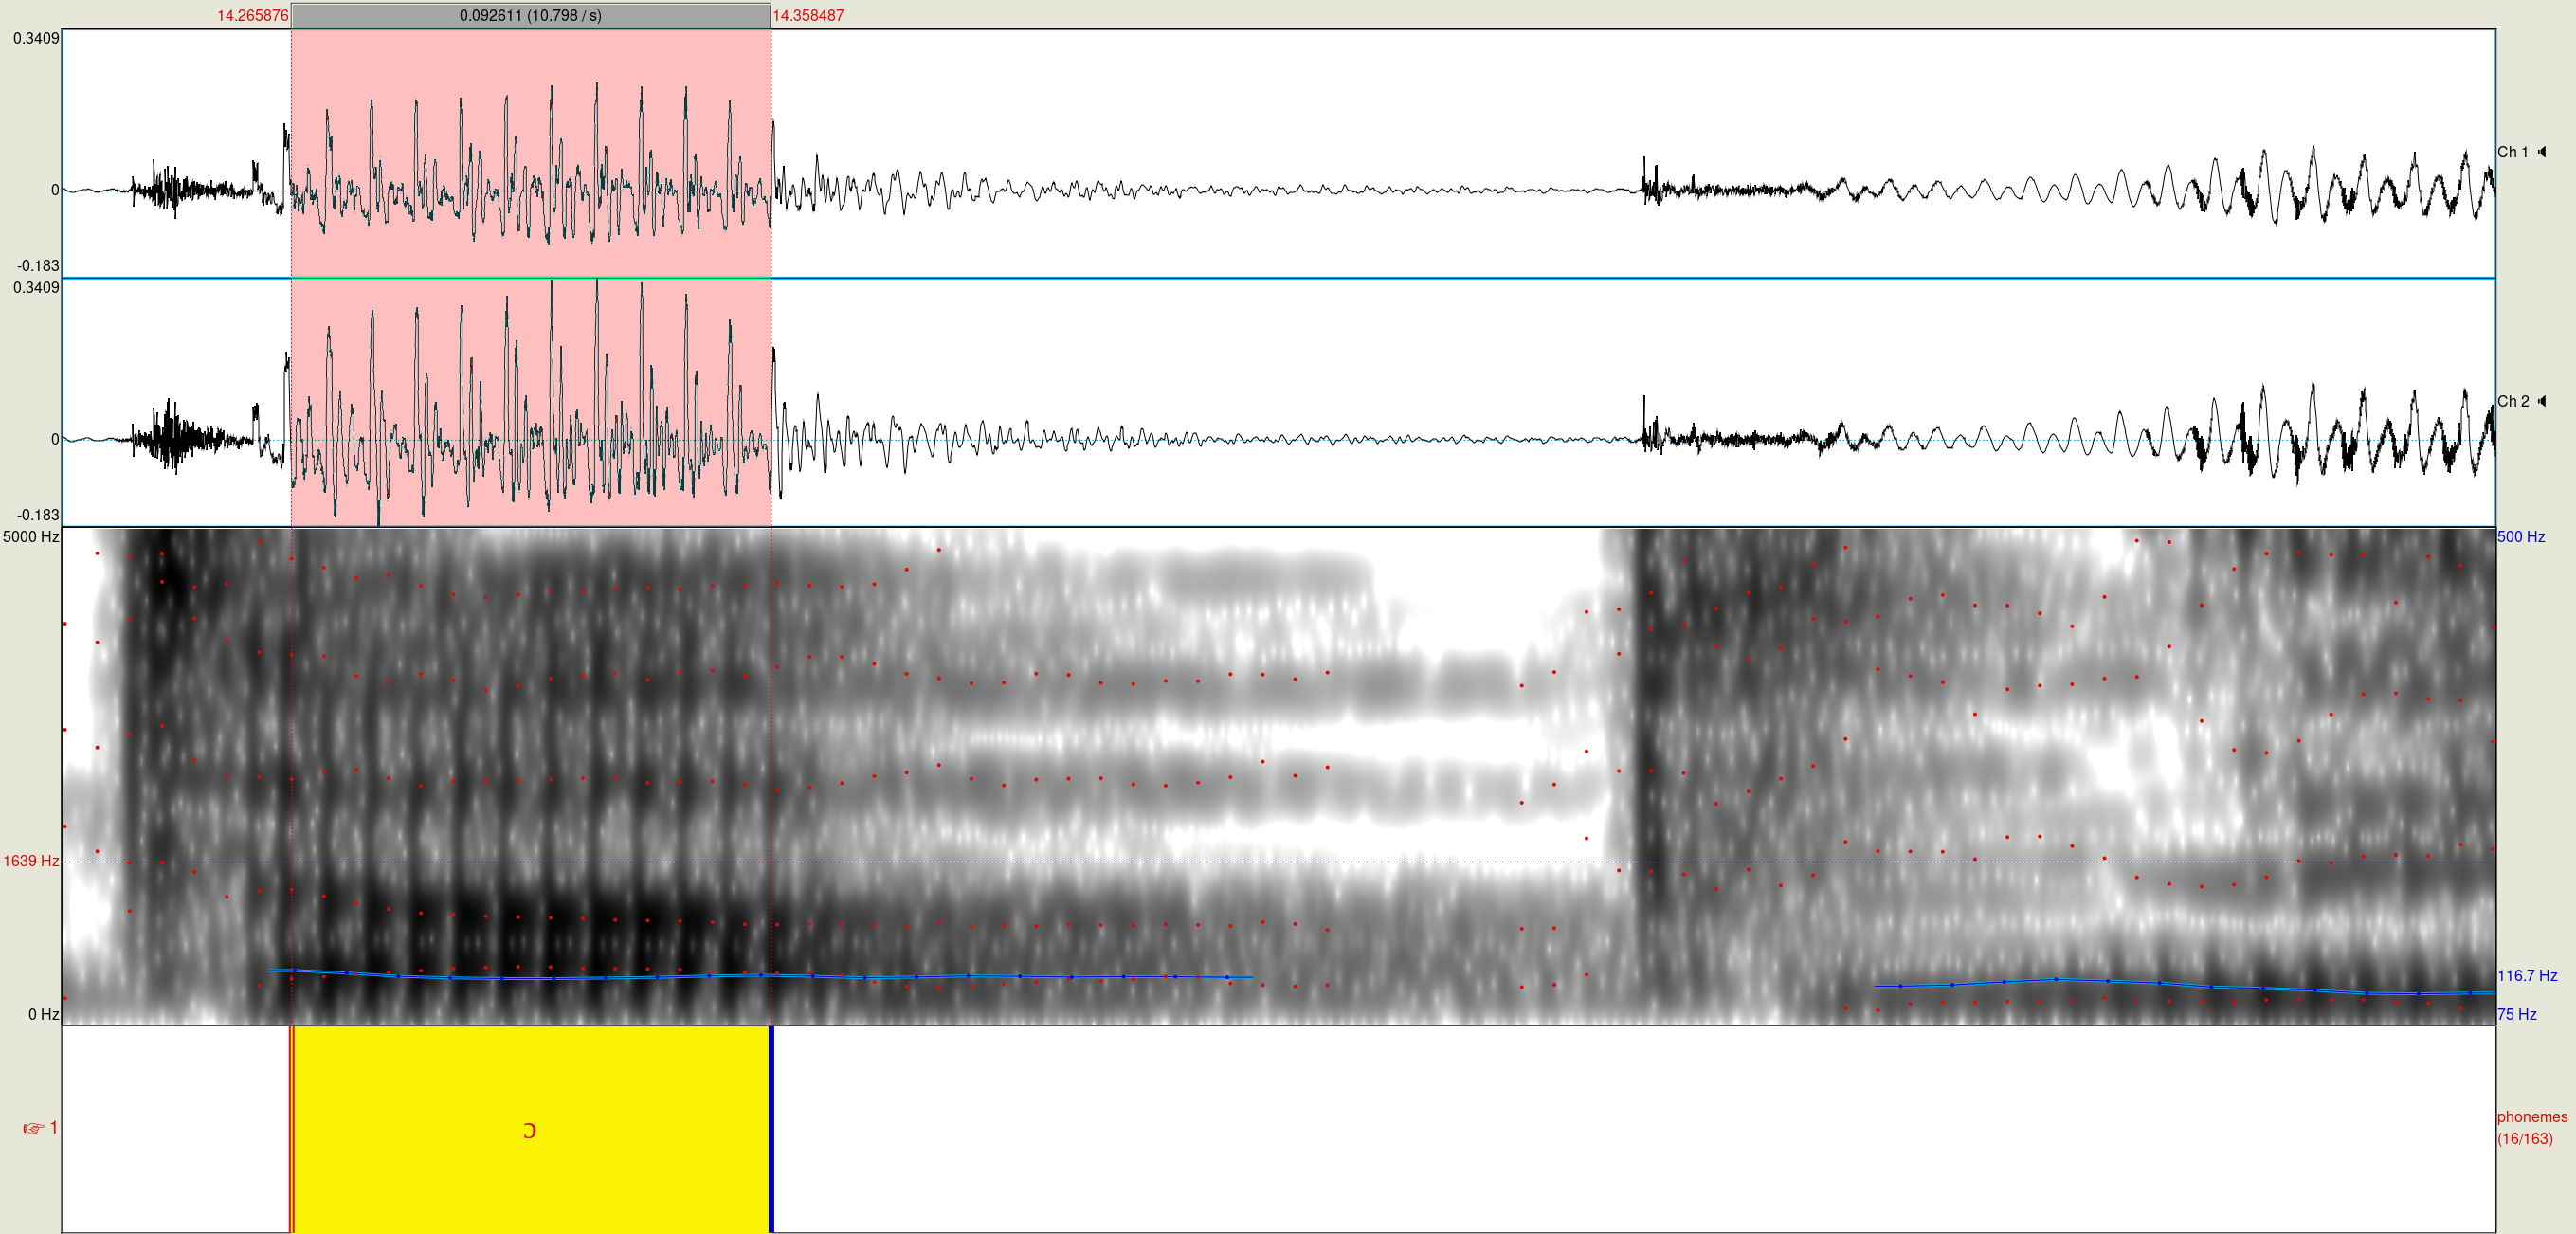
\includegraphics[width=0.6\linewidth]{figs/tope-ep}
    \caption{The phoneme /\textipa{O}/ tagged in the word ``tope`` /\textipa{tOp(I)}/ (summit) as spoken by the Portuguese informant. Note that the realization of the phoneme /\textipa{I}/ after the burst /\textipa{p}/ is completely missing.}
    \label{fig:tope-ep}
\end{figure}

As a result, the data tagging stage ended up with the generation of one \texttt{TextGrid} for each wavefile which includes annotations of the vowels that will be considered in this study.

\subsubsection{Automatic processing}

The tagging process carried out as explained in the previous section allows the extraction of vowel features in a  completely automatic fashion. In order to  reliably measure vowel formants and lengths is important to tune the algorithms that \texttt{praat} uses internally to extract features. The algorithms and parameters (the full script can be found in Appendix \ref{ap:script}) used to automatically extract information are discussed below.

First, the \texttt{praat} script sets off by initializing the formant and pitch structures used internally to store the data. Formants are extracted using the Burg algorithm described in \cite{childers1978modern}, which is directly available in \texttt{praat}. The algorithm was configured to take time steps corresponding to the 25 \% of the window length (0.025 seconds) and forced to search for five formants in the range from 50 to 5000 Hz (the normal range for a adult male speaker). On the other hand, the Pitch algorithm (which extracts F0) works by seeking acoustic periodicity based on the accurate auto-correlation method described in  \cite{boersma1993accurate}, which is specially suitable for the study of short vowels. It was tuned with a time step of 0.01 seconds and a floor and ceiling pitch of 60 and 400 Hz (again, the regular and recommended values form adult male speakers), respectively. Secondly, the script iteratively measures phone lengths by subtracting the end and start boundaries of each frame in the \texttt{TextGrid} structure. Then, for each phone, another loop measures the first five formants and the pitch in intervals of 0.01 seconds. This information is finally appended into a comma separated value file (CSV) for further processing outside \texttt{praat}. An extract of this CSV file can be seen in the Table \ref{tab:praat}.

     \begin{table}[htbp]
         \small
         \begin{center}
             \begin{tabular}{lcrrrrrrrr}
                 \toprule
                 \multicolumn{1}{l}{\textbf{id}} & \textbf{Phone} & \multicolumn{1}{l}{\textbf{Time}} & \multicolumn{1}{l}{\textbf{Duration}} & \multicolumn{1}{c}{\textbf{F0}} & \multicolumn{1}{c}{\textbf{F1}} & \multicolumn{1}{c}{\textbf{F2}} & \multicolumn{1}{c}{\textbf{F3}} & \multicolumn{1}{c}{\textbf{F4}} & \multicolumn{1}{c}{\textbf{F5}} \\ \midrule
                 1 & /i/ & 3.291 & 0.057 & 127.46 & 310.79 & 2,030.81 & 2,811.06 & 3,324.67 & \multicolumn{1}{l}{--undef--} \\ 
                 1 & /i/ & 3.301 & 0.057 & 127.69 & 311.28 & 2,039.91 & 2,828.94 & 3,363.13 & \multicolumn{1}{l}{--undef--} \\ 
                 1 & /i/ & 3.311 & 0.057 & 127.82 & 308.29 & 2,032.86 & 2,856.80 & 2,972.97 & 3,407.81 \\ 
                 1 & /i/ & 3.321 & 0.057 & 128.11 & 304.86 & 2,018.22 & 2,822.37 & 2,886.69 & 3,432.62 \\ 
                 1 & /i/ & 3.331 & 0.057 & 128.56 & 304.65 & 2,025.84 & 2,811.03 & 3,086.13 & 3,432.30 \\ 
                 2 & \textipa{/O/} & 3.490 & 0.045 & 137.60 & 407.28 & 1,710.13 & 2,453.89 & 3,410.83 & 3,665.35 \\ 
                 2 & \textipa{/O/} & 3.500 & 0.045 & 136.78 & 405.12 & 1,671.87 & 2,434.66 & 3,408.30 & 3,807.26 \\ 
                 2 & \textipa{/O/} & 3.510 & 0.045 & 134.75 & 396.97 & 1,614.77 & 2,420.70 & 3,408.37 & 3,533.24 \\ 
                 \bottomrule
             \end{tabular}
         \end{center}
         \caption{Extract of the first 9 elements produced by the script using \texttt{praat}.}
         \label{tab:praat}
     \end{table}
 
As it can be seen, the column \texttt{id} uniquely identifies each phone in the wavefile (in the example above, five measures of a phone /i/ are shown). The columns ``phone'', ``time'' and ``duration'' describe the phone at stake, the exact timestamp of the measurement from the beginning of the recording and the duration of the phone, respectively. The remaining columns refer to the pitch (F0) and the first five formants (F1, F2, F3, F4 and F5) measured at the corresponding timestamp. The amount of information yielded by this table is large, so further processing is needed to extract valuable data to work with. With this intention, another script in python is fed with tables as the one shown in Table \ref{tab:praat} and calculates the mean, standard deviation, median as well as the Q1 and Q3 quartiles of the vowel lengths for each phone, namely for each \texttt{id}. The script also manages the occurrences of ``--undef--'' data in the table by setting it to a neighbor value or deleting the whole row.% In Table \ref{tab:praatmedian} an example which the median values of each vowel can be seen.
 
%\begin{table}[htpb]
%    \small
%    \begin{center}
%        \begin{tabular}{lcrrrrrr}
%            \toprule
%            \textbf{id} & \multicolumn{1}{r}{\textbf{Phone}} & \textbf{Time} & \textbf{Duration} & \multicolumn{1}{c}{\textbf{F0}} & \multicolumn{1}{c}{\textbf{F1}} & \multicolumn{1}{c}{\textbf{F2}} & \multicolumn{1}{c}{\textbf{F3}} \\ \midrule
%            1 & \textipa{/i/} & 3.316 & 0.057 & 127.97 & 306.57 & 2,028.33 & 2,816.72 \\ 
%            2 & \textipa{/I/} & 3.510 & 0.045 & 134.75 & 396.97 & 1,614.77 & 2,420.70 \\ 
%            3 & /o/ & 5.170 & 0.118 & 122.34 & 402.17 & 1,058.25 & 2,527.41 \\ 
%            4 & \textipa{/U/} & 5.330 & 0.064 & 122.66 & 395.70 & 1,258.02 & 2,378.94 \\ 
%            \bottomrule
%        \end{tabular}
%    \end{center}
%    \caption{Extract of the first five median values of some instances of the phones /\textipa{i, I, o, U, a}/.}
%    \label{tab:praatmedian}
%\end{table}




\section{Results}

The aim of this section is to analyze the acoustic measurements carried out as detailed in the previous section, being the main goal to find the differences between the Galician-Portuguese varieties in terms of the first two formants and length of vowels. More in detail, this section is divided in three subsections: the first one describes the data collected, the second one describes the results for formants and finally the results of vowel duration are discussed.

\subsection{Data}
Table~\ref{tab:data} summarizes the vowel duration and formant measurements by average and standard deviation values. 
\begin{table}[htb]
    \def\arraystretch{1.3}% 
    \begin{center}
        \scriptsize
        \scalebox{0.896}{
        \begin{tabular}{llrrrrrrrrrr}
            \toprule
            \multicolumn{ 2}{l}{\textbf{Phone}} & \multicolumn{1}{c}{\textipa{/i/}} & \multicolumn{1}{c}{\textipa{/I/}} & \multicolumn{1}{c}{\textipa{/e/}} & \multicolumn{1}{c}{\textipa{/E/}} & \multicolumn{1}{c}{\textipa{/a/}} & \multicolumn{1}{c}{\textipa{/5/}} & \multicolumn{1}{c}{\textipa{/o/}} & \multicolumn{1}{c}{\textipa{/O/}} & \multicolumn{1}{c}{\textipa{/u/}} & \multicolumn{1}{c}{\textipa{/U/}} \\ \midrule
            \multicolumn{ 1}{l}{\textbf{Galician}} & \multicolumn{ 1}{l}{Dur.} & 71.97 & 57.17 & 82.93 & 96.06 & 96.13 & 65.85 & 84.67 & 86.17 & 96.17 & 61.23 \\ 
            \multicolumn{ 1}{l}{} & \multicolumn{ 1}{l}{} & $\mypm$14.67 & $\mypm$10.33 & $\mypm$14.32 & $\mypm$9.83 & $\mypm$21.10 & $\mypm$14.38 & $\mypm$21.79 & $\mypm$11.08 & $\mypm$0.0 & $\mypm$12.94 \\[0.5em]
            \multicolumn{ 1}{l}{} & \multicolumn{ 1}{l}{F0} & 120.53 & 124.59 & 119.73 & 110.84 & 112.36 & 123.65 & 116.97 & 111.78 & 122.76 & 125.11 \\ 
            \multicolumn{ 1}{l}{} & \multicolumn{ 1}{l}{} & $\mypm$3.85 & $\mypm$5.54 & $\mypm$4.51 & $\mypm$3.13 & $\mypm$5.54 & $\mypm$5.04 & $\mypm$3.71 & $\mypm$2.60 & $\mypm$0.00 & $\mypm$6.42 \\[0.5em]
            \multicolumn{ 1}{l}{} & \multicolumn{ 1}{l}{F1} & 291.73 & 391.61 & 414.76 & 504.76 & 669.56 & 450.54 & 446.21 & 510.22 & 359.52 & 393.00 \\ 
            \multicolumn{ 1}{l}{} & \multicolumn{ 1}{l}{} & $\mypm$14.63 & $\mypm$66.86 & $\mypm$22.74 & $\mypm$64.65 & $\mypm$31.47 & $\mypm$35.78 & $\mypm$27.86 & $\mypm$18.81 & $\mypm$0.00 & $\mypm$37.50 \\[0.5em]
            \multicolumn{ 1}{l}{} & \multicolumn{ 1}{l}{F2} & 1,987.74 & 1,680.62 & 1,793.93 & 1,645.22 & 1,393.02 & 1,501.81 & 984.87 & 1,013.79 & 1,064.47 & 1,360.25 \\ 
            \multicolumn{ 1}{l}{} & \multicolumn{ 1}{l}{} & $\mypm$76.26 & $\mypm$83.78 & $\mypm$87.95 & $\mypm$93.21 & $\mypm$66.81 & $\mypm$56.92 & $\mypm$82.91 & $\mypm$9.96 & $\mypm$0.00 & $\mypm$118.50 \\[0.5em]
            \multicolumn{ 1}{l}{} & \multicolumn{ 1}{l}{F3} & 2,755.38 & 2,458.97 & 2,509.44 & 2,497.66 & 2,407.48 & 2,444.21 & 2,496.47 & 2,435.78 & 2,465.69 & 2,375.84 \\ 
            \multicolumn{ 1}{l}{} & \multicolumn{ 1}{l}{} & $\mypm$183.97 & $\mypm$105.22 & $\mypm$71.07 & $\mypm$77.27 & $\mypm$49.33 & $\mypm$103.74 & $\mypm$83.33 & $\mypm$13.00 & $\mypm$0.00 & $\mypm$101.38 \\[1em]
            \multicolumn{ 1}{l}{\textbf{EP}} & \multicolumn{ 1}{l}{Dur.} & 73.42 & 35.22 & 93.75 & 92.02 & 102.93 & 55.56 & 89.79 & 94.25 & 58.04 & 36.46 \\ 
            \multicolumn{ 1}{l}{} & \multicolumn{ 1}{l}{} & $\mypm$14.59 & $\mypm$2.81 & $\mypm$16.63 & $\mypm$19.29 & $\mypm$16.82 & $\mypm$11.83 & $\mypm$32.67 & $\mypm$26.33 & $\mypm$0.00 & $\mypm$3.16 \\[0.5em]
            \multicolumn{ 1}{l}{} & \multicolumn{ 1}{l}{F0} & 120.09 & 106.02 & 119.76 & 117.64 & 116.28 & 113.55 & 116.59 & 115.58 & 121.58 & 107.81 \\ 
            \multicolumn{ 1}{l}{} & \multicolumn{ 1}{l}{} & $\mypm$5.53 & $\mypm$9.26 & $\mypm$3.70 & $\mypm$2.92 & $\mypm$2.45 & $\mypm$5.23 & $\mypm$2.58 & $\mypm$1.36 & $\mypm$0.00 & $\mypm$7.21 \\[0.5em]
            \multicolumn{ 1}{l}{} & \multicolumn{ 1}{l}{F1} & 287.63 & 286.97 & 377.48 & 463.70 & 589.12 & 374.88 & 470.17 & 515.37 & 314.26 & 274.56 \\ 
            \multicolumn{ 1}{l}{} & \multicolumn{ 1}{l}{} & $\mypm$19.85 & $\mypm$34.09 & $\mypm$26.32 & $\mypm$13.40 & $\mypm$34.00 & $\mypm$29.16 & $\mypm$34.04 & $\mypm$15.14 & $\mypm$0.00 & $\mypm$16.29 \\[0.5em]
            \multicolumn{ 1}{l}{} & \multicolumn{ 1}{l}{F2} & 2,124.96 & 1,602.56 & 1,932.65 & 1,788.77 & 1,426.42 & 1,707.71 & 1,020.73 & 1,065.22 & 1,145.86 & 1,672.74 \\ 
            \multicolumn{ 1}{l}{} & \multicolumn{ 1}{l}{} & $\mypm$49.40 & $\mypm$98.65 & $\mypm$65.81 & $\mypm$75.25 & $\mypm$120.62 & $\mypm$104.37 & $\mypm$155.53 & $\mypm$63.62 & $\mypm$0.00 & $\mypm$140.38 \\[0.5em]
            \multicolumn{ 1}{l}{} & \multicolumn{ 1}{l}{F3} & 2,830.45 & 2,599.37 & 2,502.11 & 2,387.64 & 2,333.16 & 2,414.42 & 2,348.96 & 2,232.19 & 2,214.53 & 2,859.37 \\ 
            \multicolumn{ 1}{l}{} & \multicolumn{ 1}{l}{} & $\mypm$174.29 & $\mypm$51.11 & $\mypm$49.23 & $\mypm$95.38 & $\mypm$102.02 & $\mypm$123.35 & $\mypm$98.70 & $\mypm$107.66 & $\mypm$0.00 & $\mypm$187.63 \\[1em]
            \multicolumn{ 1}{l}{\textbf{BP}} & \multicolumn{ 1}{l}{Dur.} & 87.45 & 51.92 & 107.78 & 118.55 & 117.76 & 54.22 & 105.34 & 109.98 & 114.26 & 59.14 \\ 
            \multicolumn{ 1}{l}{} & \multicolumn{ 1}{l}{} & $\mypm$10.01 & $\mypm$11.09 & $\mypm$41.80 & $\mypm$20.11 & $\mypm$20.46 & $\mypm$7.76 & $\mypm$26.94 & $\mypm$19.27 & $\mypm$0.00 & $\mypm$11.30 \\[0.5em]
            \multicolumn{ 1}{l}{} & \multicolumn{ 1}{l}{F0} & 163.42 & 127.33 & 153.46 & 143.55 & 137.00 & 128.68 & 148.21 & 137.98 & 162.37 & 131.97 \\ 
            \multicolumn{ 1}{l}{} & \multicolumn{ 1}{l}{} & $\mypm$10.93 & $\mypm$5.91 & $\mypm$11.78 & $\mypm$8.09 & $\mypm$6.09 & $\mypm$6.69 & $\mypm$8.42 & $\mypm$6.50 & $\mypm$0.00 & $\mypm$8.66 \\[0.5em]
            \multicolumn{ 1}{l}{} & \multicolumn{ 1}{l}{F1} & 321.55 & 334.04 & 424.04 & 544.90 & 757.97 & 412.99 & 443.85 & 601.67 & 366.57 & 348.87 \\ 
            \multicolumn{ 1}{l}{} & \multicolumn{ 1}{l}{} & $\mypm$12.29 & $\mypm$8.63 & $\mypm$27.72 & $\mypm$26.07 & $\mypm$38.45 & $\mypm$36.64 & $\mypm$23.77 & $\mypm$36.81 & $\mypm$0.00 & $\mypm$18.37 \\[0.5em]
            \multicolumn{ 1}{l}{} & \multicolumn{ 1}{l}{F2} & 2,089.60 & 1,851.80 & 1,981.08 & 1,842.57 & 1,470.22 & 1,714.27 & 946.98 & 1,070.28 & 994.70 & 1,598.20 \\ 
            \multicolumn{ 1}{l}{} & \multicolumn{ 1}{l}{} & $\mypm$104.21 & $\mypm$75.14 & $\mypm$98.21 & $\mypm$72.00 & $\mypm$72.34 & $\mypm$89.07 & $\mypm$106.26 & $\mypm$71.93 & $\mypm$0.00 & $\mypm$117.69 \\[0.5em]
            \multicolumn{ 1}{l}{} & \multicolumn{ 1}{l}{F3} & 2,773.91 & 2,753.06 & 2,614.96 & 2,624.25 & 2,365.15 & 2,620.97 & 2,535.98 & 2,354.49 & 2,428.09 & 2,416.77 \\ 
            \multicolumn{ 1}{l}{} & \multicolumn{ 1}{l}{} & $\mypm$94.29 & $\mypm$50.77 & $\mypm$100.90 & $\mypm$64.31 & $\mypm$77.84 & $\mypm$167.62 & $\mypm$80.79 & $\mypm$143.74 & $\mypm$0.00 & $\mypm$112.82 \\ \bottomrule
        \end{tabular}
    }
    \end{center}
    \caption{Average and standard deviation ($\mypm$) values of vowel duration, F0, F1, F2 and F3 for each phone and speaker of Galician, EP and BP.}
    \label{tab:data}
\end{table}

On the one hand, each table's cell is vertically divided into two subcells. The average of all the instances of the corresponding phone (indicated by the column label) spoken by a certain speaker (indicated by the left-most row label) is shown in the upper cell, whilst the standard deviation of the measures is displayed in the lower part (after the $\mypm$ symbol). On the other hand, the second left-most row label indicates the feature measured: duration (Dur. in the table) is displayed in milliseconds (ms) and the formants are measured in Hertz (Hz). 

Coarsely speaking, the data in the table show differences among the three dialects of Galician-Portuguese: the duration of the Galician vowels tend to take less extreme values than its counterparts, being the reductions shorter than the phones pronounced at the stressed syllable. This last tendency is also shown for EP and BP. In relation to the fundamental frequency, Galician and EP speakers have a similar register as opposed to the BP informant, who repeatedly  pronounced the phones with a higher pitch. This phenomenon will have an influence in the values of F1, F2 and F3 formants, as harmonics are closely related to the fundamental frequency. This data will be further analyzed in the following sections, starting with formants.

\subsection{Formant analysis}

Figure \ref{fig:formants} depicts the median F1 and F2 formant values of each phone as spoken by the informants using the regular and the plural reading lists. The whole figure is divided into six diagrams: row-wise is the representation of the different dialects and column-wise, the representation the two readings lists (non-pluralized vs. pluralized). In each one, phones are depicted with its corresponding IPA symbol using different colors, each phone representing the median of measurements of a single vowel. Note that the scale of the axis is logarithmic: this decision is motivated by the fact that the frequency perception of the human ear is not linear but follows a logarithmic curve (a comprehensive transformation could be done using the Mel scale), and that the limits of the axis are shared in all six diagrams, therefore direct comparisons between them are possible. In addition, the direction of axis have been reversed, so the final representation of the phones is displayed in accordance to the positions of the standard IPA vowel chart, where the openness of the jaw and the frontness of the tongue correspond to the first and second formants in decreasing order, respectively.\\

In relation to the formant data shown in the diagrams, it can be seen that in general all the phones, regardless of the language and reading list, lie in a position that is either in-place (in relation to the overall position in the IPA vowel chart) or shifted from its natural position but still surrounded by correct cluster phones. For instance, although the phoneme /\textipa{5}/ in the BP dataset (see Figure \ref{fig:bp} or Figure \ref{fig:bps}) appears to be shifted to the upper-left corner according to IPA (reminding even to the position of the \textipa{/@/} phoneme), its relative position (central, surrounded by all the remainder phones) is still correct. Equally noticeable is the fact that the range of the formants differs among the dialects. BP tends to use all the available spectrum:  the ratio of the openness and closeness of the jaw when producing, e.g. the phones /\textipa{i, a}/, is in general wider than EP and much wider than Galician. This tendency is also observed regarding the frontness/backness aspect of the tongue, being BP the greatest exponent and Galician the most relaxed one. In this sense, it looks like the influence of the Spanish language (which only accounts for five different realization of vowels /\textipa{a, e, i, o, u}/) had a toll on the Galician pronunciation. This theory is supported not only by the overall vocalic range, but also in that the distances of pairs /\textipa{e}/ vs. /\textipa{E}/ and /\textipa{o}/ vs. /\textipa{O}/ is much shorter (and thus the distinction is vaguer) than its counterparts (compare Figures \ref{fig:gl} and \ref{fig:ep}). In addition, it can be noticed that the nasalization of vowels (annotated in the BP chart in Figures \ref{fig:bp} and \ref{fig:bps}) do not have an impact in the place of articulation whatsoever. \\


%hacer los ratio para ver las distinciones entre idiomas.
%las nasales no afectan.

     
%\begin{tikzpicture}
%\begin{axis}[
% x dir=reverse,
%  y dir=reverse,
%  grid = both,
%%  ymode=log,
%%  log basis y={50}
%  ]
%
%\addplot [
%point meta=explicit symbolic,
%scatter, only marks,
%mark=text,
%scatter/@pre marker code/.code={\pgfplotsset{text mark=\textipa{\pgfplotspointmeta}}},
%scatter/@post marker code/.code={}
%] table [x=F2, 
%y=F1, 
%col sep=comma,
%meta=phoneme] {data/julio/p1.mean.csv};
%
%
%\end{axis}
%
%\end{tikzpicture}

\begin{figure}
\def\minx{650}
\def\minxstep{700}

\subfloat[]{\noindent
\begin{tikzpicture}
\begin{axis}[
title=Brazilian Portuguese,
xmode=log,
width=7.6cm,
ylabel=F1 (Hz),
xlabel=F2 (Hz),
ymode=log,
log basis y={2},
x dir=reverse,
y dir=reverse,
xmin=\minx,
xmax=2500,
ymin=200,
ymax=850,
extra y tick style={%
    fill=white,
    label=none,
    draw=none,
    tickwidth=0.8mm,
    fill opacity=0,
},
extra x tick style={%
    fill=white,
    label=none,
    draw=none,
    tickwidth=0.8mm,
    fill opacity=0,
},
ytick={200,300,500,800},
xtick={\minx,900,1200,1800, 2500},,
extra y ticks={200,210,...,850},
extra x ticks={\minx,\minxstep,...,2500},
yminorticks=true,
log ticks with fixed point,
]

\plotallphonemes{data/julio/p1.median.csv}

\end{axis}
\end{tikzpicture}\label{fig:bp}} \subfloat[]{\begin{tikzpicture}
\begin{axis}[
title=Brazilian Portuguese (plurals),
xmode=log,
width=7.6cm,
ylabel=F1 (Hz),
xlabel=F2 (Hz),
ymode=log,
log basis y={2},
x dir=reverse,
y dir=reverse,
xmin=\minx,
xmax=2500,
ymin=200,
ymax=850,
extra y tick style={%
    fill=white,
    label=none,
    draw=none,
    tickwidth=0.8mm,
    fill opacity=0,
},
extra x tick style={%
    fill=white,
    label=none,
    draw=none,
    tickwidth=0.8mm,
    fill opacity=0,
},
ytick={200,300,500,800},
xtick={\minx,900,1200,1800, 2500},
extra y ticks={200,210,...,850},
extra x ticks={\minx,\minxstep,...,2500},
yminorticks=true,
log ticks with fixed point,
]

\plotallphonemes{data/julio/p2.median.csv}

\end{axis}
\end{tikzpicture}\label{fig:bps}}


\subfloat[]{\noindent\begin{tikzpicture}
\begin{axis}[
title=Galician,
xmode=log,
width=7.6cm,
ylabel=F1 (Hz),
xlabel=F2 (Hz),
ymode=log,
log basis y={2},
x dir=reverse,
y dir=reverse,
xmin=\minx,
xmax=2500,
ymin=200,
ymax=850,
extra y tick style={%
    fill=white,
    label=none,
    draw=none,
    tickwidth=0.8mm,
    fill opacity=0,
},
extra x tick style={%
    fill=white,
    label=none,
    draw=none,
    tickwidth=0.8mm,
    fill opacity=0,
},
ytick={200,300,500,800},
xtick={\minx,900,1200,1800, 2500},,
extra y ticks={200,210,...,850},
extra x ticks={\minx,\minxstep,...,2500},
yminorticks=true,
log ticks with fixed point,
]

\plotallphonemes{data/pedro/p1.median.csv}

\end{axis}
\end{tikzpicture}\label{fig:gl}}\subfloat[]{\begin{tikzpicture}
\begin{axis}[
title=Galician (plurals),
xmode=log,
width=7.6cm,
ylabel=F1 (Hz),
xlabel=F2 (Hz),
ymode=log,
log basis y={2},
x dir=reverse,
y dir=reverse,
xmin=\minx,
xmax=2500,
ymin=200,
ymax=850,
extra y tick style={%
    fill=white,
    label=none,
    draw=none,
    tickwidth=0.8mm,
    fill opacity=0,
},
extra x tick style={%
    fill=white,
    label=none,
    draw=none,
    tickwidth=0.8mm,
    fill opacity=0,
},
ytick={200,300,500,800},
xtick={\minx,900,1200,1800, 2500},,
extra y ticks={200,210,...,850},
extra x ticks={\minx,\minxstep,...,2500},
yminorticks=true,
log ticks with fixed point,]

\plotallphonemes{data/pedro/p2.median.csv}

\end{axis}
\end{tikzpicture}\label{fig:gls}}

\subfloat[]{\noindent
\begin{tikzpicture}
\begin{axis}[
title=European Portuguese,
xmode=log,
width=7.6cm,
ylabel=F1 (Hz),
xlabel=F2 (Hz),
ymode=log,
log basis y={2},
x dir=reverse,
y dir=reverse,
xmin=\minx,
xmax=2500,
ymin=200,
ymax=850,
extra y tick style={%
    fill=white,
    label=none,
    draw=none,
    tickwidth=0.8mm,
    fill opacity=0,
},
extra x tick style={%
    fill=white,
    label=none,
    draw=none,
    tickwidth=0.8mm,
    fill opacity=0,
},
ytick={200,300,500,800},
xtick={\minx,900,1200,1800, 2500},,
extra y ticks={200,210,...,850},
extra x ticks={\minx,\minxstep,...,2500},
yminorticks=true,
log ticks with fixed point,
]

\plotallphonemes{data/joao/p1.median.csv}

\end{axis}
\end{tikzpicture}\label{fig:ep}}\subfloat[]{\begin{tikzpicture}
\begin{axis}[
title=European Portuguese (plurals),
xmode=log,
width=7.6cm,
ylabel=F1 (Hz),
xlabel=F2 (Hz),
ymode=log,
log basis y={2},
x dir=reverse,
y dir=reverse,
xmin=\minx,
xmax=2500,
ymin=200,
ymax=850,
extra y tick style={%
    fill=white,
    label=none,
    draw=none,
    tickwidth=0.8mm,
    fill opacity=0,
},
extra x tick style={%
    fill=white,
    label=none,
    draw=none,
    tickwidth=0.8mm,
    fill opacity=0,
},
ytick={200,300,500,800},
xtick={\minx,900,1200,1800, 2500},,
extra y ticks={200,210,...,850},
extra x ticks={\minx,\minxstep,...,2500},
yminorticks=true,
log ticks with fixed point,]

\plotallphonemes{data/joao/p2.median.csv}

\end{axis}
\end{tikzpicture}\label{fig:eps}}

\caption{First and second formants of the Brazilian, Galician and Portuguese speakers.}
\label{fig:formants}

\end{figure}

     
Another key point is the place of articulation of reductions, which apparently have different behaviors in all three dialects. Let us approach the analysis language-wise. The reductions as produced by the Brazilian informant are placed in a very high position and slightly shifted to the left. There is a clear distinction between the cluster of the phone /\textipa{5}/ and the cluster consisting of both phones /\textipa{I, U}/, having phones of the latter cluster the tendency to be mixed.  On the contrary, the place of articulation of Galician reductions is much lower (around the place of articulation of /\textipa{@}/) and condensed in a very small amount of space. Finally, the EP shows the lack of reductions from the vowel ``o'' to the phone /\textipa{U}/ and specially from the vowel ``e'' to the phone /\textipa{I}/. This is caused because most reductions of these vowels were not audible at all (a further discussion of this phenomenon is provided in the next section), thus the phone /\textipa{U}/ is scattered all around the upper part of the diagram due to unreliable measurements. In contrast, the EP speaker produces the phone /\textipa{5}/ as expected, but their mean values lie somewhere between the place of articulation of Galician and BP. Lastly, it is worth noting that the place of articulation of reductions does not appear to change significantly when words are pluralized (EP and BP add the phoneme /\textipa{S}/, in Galician, the phoneme /s/), i.e. when sibilants are added to codas of non-stressed syllables. As a summary of Figure \ref{fig:formants}, the complete vowel spaces of the three dialects are shown in Figure \ref{fig:mean}. Each point is calculated as the mean of all vowels measured in the readings lists. Those who correspond to the symmetrical vowels are connected through a line, which allows the visualization of the area embraced by each dialect's vowel space.  It can be seen that all the tendencies described above match the summarized results and supports the overall impression that from the point of view of native Galician speakers, BP's vowels are ``wider'' than EP's.
     %\begin{tikzpicture}
%\begin{axis}[
%ylabel=F1 (Hz),
%xlabel=F2 (Hz),
%ymode=log,
%log basis y={2},
%x dir=reverse,
%y dir=reverse,
%xmin=850,
%xmax=2100,
%ymin=250,
%ymax=750,
%extra y tick style={%
%    fill=white,
%    label=none,
%    draw=none,
%    tickwidth=0.8mm,
%    fill opacity=0,
%},
%ytick={200,300,500,800},
%extra y ticks={200,210,...,850},
%yminorticks=true,
%log ticks with fixed point,
%]
%
%\addplot [
%point meta=explicit symbolic,
%scatter, only marks,
%mark=text,
%scatter/@pre marker code/.code={\pgfplotsset{text mark=\colorbox{white}{\textipa{\pgfplotspointmeta}}}},
%scatter/@post marker code/.code={}
%] table [x=F2, 
%y=F1, 
%col sep=comma,
%meta=phoneme] {data/pedro/p1.mean.summary.csv};
%
%\addplot [
%black,
%] table [x=F2, 
%y=F1, 
%col sep=comma,
%meta=phoneme] {data/pedro/p1.mean.summary_7.csv};
%
%
%\end{axis}
%
%\end{tikzpicture}
\begin{figure}[htpb]
\noindent
\begin{tikzpicture}
\begin{axis}[
width=\textwidth,
height=10cm,
ylabel=F1 (Hz),
xlabel=F2 (Hz),
xmode=log,
ymode=log,
log basis y={2},
x dir=reverse,
y dir=reverse,
xmin=650,
xmax=2300,
ymin=250,
ymax=850,
extra y tick style={%
    fill=white,
    label=none,
    draw=none,
    tickwidth=0.8mm,
    fill opacity=0,
},
extra x tick style={%
    fill=white,
    label=none,
    draw=none,
    tickwidth=0.8mm,
    fill opacity=0,
},
ytick={200,300,500,800},
extra y ticks={200,210,...,850},
xtick={650,900,1200,1700, 2300},
extra x ticks={650,700,...,2500},
yminorticks=true,
log ticks with fixed point,
legend entries = {Galician, Brazilian Portuguese, European Portuguese},
legend to name={legend},
legend columns=3,
legend style={/tikz/every even column/.append style={column sep=0.3cm}},
name=border,
]

\addlegendimage{blue,densely dashed,mark=text, text mark=\colorbox{white}{\makebox[0.0em]{\textipa{O}}}}
\addlegendimage{red,mark=text, text mark=\colorbox{white}{\makebox[0.0em]{\textipa{O}}}}
\addlegendimage{n11,densely dotted,
    thick,mark=text, text mark=\colorbox{white}{\makebox[0.0em]{\textipa{O}}}}

\addplot [
blue!70!black,
point meta=explicit symbolic,
scatter, only marks,
mark=text,
scatter/@pre marker code/.code={\pgfplotsset{text mark=\colorbox{white}{\makebox[0.0em]{\textipa{\pgfplotspointmeta}}}}},
scatter/@post marker code/.code={}
] table [x=F2, 
y=F1, 
col sep=comma,
meta=phoneme] {data/pedro/p1.mean.summary.csv};

\addplot [
blue, densely dashed,
] table [x=F2, 
y=F1, 
col sep=comma,
meta=phoneme] {data/pedro/p1.mean.summary_7.csv};

\addplot [
red!70!black,
point meta=explicit symbolic,
scatter, only marks,
mark=text,
scatter/@pre marker code/.code={\pgfplotsset{text mark=\colorbox{white}{\makebox[0.0em]{\textipa{\pgfplotspointmeta}}}}},
scatter/@post marker code/.code={}
] table [x=F2, 
y=F1, 
col sep=comma,
meta=phoneme] {data/julio/p1.mean.summary.csv};

\addplot [
red,
] table [x=F2, 
y=F1, 
col sep=comma,
meta=phoneme] {data/julio/p1.mean.summary_7.csv};


\addplot [
n11!70!black,
point meta=explicit symbolic,
scatter, only marks,
mark=text,
scatter/@pre marker code/.code={\pgfplotsset{text mark=\colorbox{white}{\makebox[0.0em]{\textipa{\pgfplotspointmeta}}}}},
scatter/@post marker code/.code={}
] table [x=F2, 
y=F1, 
col sep=comma,
meta=phoneme] {data/joao/p1.mean.summary.csv};

\addplot [
densely dotted,
thick,
n11,
] table [x=F2, 
y=F1, 
col sep=comma,
meta=phoneme] {data/joao/p1.mean.summary_7.csv};

\legend{Galician,Brazilian Portuguese,European Portuguese}

\end{axis}

\node[below] at ([yshift=-1.4cm]border.south) {\ref{legend}};

\end{tikzpicture}
\caption{Mean values of the first and second formants as realized by each speaker.}
\label{fig:mean}
\end{figure}
     
     
 That being said, it is well known that the influence of a specific articulation must be expressed as a ratio of the formants rather than the difference between them. In this sense, The Formant Ratio Theory  \cite{pottersteinberg} states that vowels categories can be characterized by the formant ratio, independently from the absolute formant frequencies. Although this theory has been challenged recently \cite{johnoson}, other authors suggest that there is enough statistical evidence \cite{ratio} to consider the formant ratio as a valid measure of vowel categorization. Given this, it is possible to use the ratio as a measure of distance between vowel types. In other words, the same vowel category produced by two different speakers must have some certain F1 and F2 values such that the ratio among them is constant. The opposite can be said about vowels with two distant ratio measurements: the larger the distance, the more different the vowel categories are. For this study, this approach can be used to characterize, as far as the formants are concerned, how distant vowel categories are between the pairs of dialects at stake. This is done by considering the ratio of phones as continuous value of a signal (which can be though as a fingerprint of the vowels of a language), therefore each language has a different spectrum that only depends on the ratio of their formants. The distance between these signals  can be computed in terms of the simplest correlation method:
 \begin{equation}\label{eq:distance}
     \delta = \sum_{p \in {P}} \sqrt{(r_p^{(1)}-r_p^{(2)})^2}, \quad P = \{\text{\textipa{i, I, e, E, a, 5, o, O, u, U}}\},
 \end{equation}
 
 \noindent where $r_p^{(1)}$ and $r_p^{(2)}$ are the formant ratios of phone $p$ in target languages (1) and (2), respectively. In Table \ref{fig:distance} are shown the phone-wise distances in terms of  F1/F2, F1/F3 and F2/F3 ratios as well as the $\delta$ value between pairs of dialects, following the Equation \eqref{eq:distance}.
     \begin{table}[htbp]
        \def\arraystretch{1.3}% 
\begin{center}
        \small
\begin{tabular}{llrrrrrrrrrrr}
	\toprule
    \textbf{Phone} &  & \multicolumn{1}{c}{\textipa{/i/}} & \multicolumn{1}{c}{\textipa{/I/}} & \multicolumn{1}{c}{\textipa{/e/}} & \multicolumn{1}{c}{\textipa{/E/}} & \multicolumn{1}{c}{\textipa{/a/}} & \multicolumn{1}{c}{\textipa{/5/}} & \multicolumn{1}{c}{\textipa{/o/}} & \multicolumn{1}{c}{\textipa{/O/}} & \multicolumn{1}{c}{\textipa{/u/}} & \multicolumn{1}{c}{\textipa{/U/}} & \multicolumn{1}{c}{\textbf{$\delta$}} \\ \midrule
	F2/F1 & G-EP  & 0.57 & 1.29 & 0.79 & 0.60 & 0.34 & 1.22 & 0.04 & \textbf{0.08} & 0.69 & 2.63 &          8.26 \\
	      & G-BP      & \textbf{0.31} & 1.25 & \textbf{0.35} & \textbf{0.12} & \textbf{0.14} & 0.82 & 0.07 & 0.21 & \textbf{0.25} & \textbf{1.12} & \textbf{4.64} \\
	      & BP-EP    & 0.89 & \textbf{0.04 }& 0.45 & 0.48 & 0.48 & \textbf{0.40} & \textbf{0.04} & 0.29 & 0.93 & 1.51 &          5.51 \\[0.5em]
          
	F3/F1 & G-EP  & \textbf{0.40} & 2.78 & 0.58 & 0.20 & \textbf{0.36} & 1.02 & 0.60 & 0.44 & \textbf{0.19} & 4.37 &         10.93 \\
	      & G-BP      & 0.82 & 1.96 & \textbf{0.12} & \textbf{0.13} & 0.48 & 0.92 & \textbf{0.12} & 0.86 & 0.23 & \textbf{0.88} & \textbf{6.52} \\
	      & BP-EP    & 1.21 & \textbf{0.82} & 0.46 & 0.33 & 0.84 & \textbf{0.09} & 0.72 & \textbf{0.42} & 0.42 & 3.49 &          8.80 \\[0.5em]
          
	F3/F2 & G-EP  & 0.05 & 0.16 & 0.10 & 0.18 & 0.09 & 0.21 & 0.23 & 0.31 & 0.38 & \textbf{0.04} &          1.77 \\
	      & G-BP      & 0.06 & \textbf{0.02} & 0.08 & \textbf{0.09} & 0.12 & \textbf{0.10} & \textbf{0.14} & 0.20 & \textbf{0.12} & 0.23 & \textbf{1.18} \\
	      & BP-EP    & \textbf{0.00} & 0.14 & \textbf{0.03} & 0.09 & \textbf{0.03} & 0.12 & 0.38 & \textbf{0.10} & 0.51 & 0.20 &          1.58 \\ \bottomrule
\end{tabular}
\end{center}
\caption{Phone-wise distance between Galician, EP and BP languages. The higher the value, the more distant.}
\label{fig:distance}
\end{table}

     
  As it can be seen, the Galician-BP (G-BP in the table) is the pair of dialects with the lowest overall distance independently of the formant ratio used (e.g. 4.62 vs. 5.51 for BP-EP and 4.62 vs. 8.26 yielded for the G-EP combination using the F1/F2 ratio). However, it must be taken into account that, although these results can lead to the conclusion that the vowel types of the combination G-BP are the closest, the measurements of F2 and F3 are not as reliable as F1 (shown by the standard deviation metric in Table \ref{tab:data}) and the number of participants is not statistically relevant. With that in mind, it is true that this first empirical evidence from formants support that the degree of understanding between Galician and BP is higher than any other combination, as the overall place of articulation of vowels is the closest.
  
  \subsection{Duration analysis}
  
Apart from the point of articulation, the duration of vowels can be a key characteristic in some languages in that the distinction between words are not only based on the openness of the jaw and frontness of the tongue but also in the length of the vowel itself, as it is the case for instance in German. As mentioned in the introduction, none of the languages considered in this study
use a vowel system which includes the vowel length as phonological feature.
\begin{figure}[htpb]
    \centering
\noindent
\begin{tikzpicture}
\pgfplotstableread[col sep = comma]{data/pedro/p1.boxplot.csv}\datatablepedro
\pgfplotstableread[col sep = comma]{data/julio/p1.boxplot.csv}\datatablejulio
\pgfplotstableread[col sep = comma]{data/joao/p1.boxplot.csv}\datatablejoao
\begin{axis}[
title=Singular reading list,
ymin=0.02,
ymax=0.18,
ymajorgrids,
ylabel=Length (s),
xlabel=Phone,
y tick label style={
    /pgf/number format/fixed,
},
typeset ticklabels with strut,
legend entries = {Galician, Brazilian Portuguese, European Portuguese},
legend to name={legend},
name=border,
legend columns=3,
legend style={/tikz/every even column/.append style={column sep=0.3cm}},
height=10cm,
width=\textwidth,
boxplot/draw direction=y,
xtick = {1, 2, 3, 4,5,6,7,8,9},
xticklabel style = {align=center},
xticklabels = {\textipa{/5/},\textipa{/E/},\textipa{/I/},\textipa{/O/},\textipa{/U/},\textipa{/a/},\textipa{/e/},\textipa{/i/},\textipa{/o/},\textipa{/u/}},
boxplot={
    %
    % Idea: 
    %  place the 
    %  group 1 at 0.3333 and 0.6666
    %  group 2 at 1.3333 and 1.6666
    %  group 3 at 2.3333 and 2.6666
    %  ...
    % in a formular:
    draw position={0.78 + floor(\plotnumofactualtype/3) + 1/4.5*fpumod(\plotnumofactualtype,3)},
    %
    % that means the box extend must be at most 0.33333 :
    box extend=0.2,
},
% ... it also means that 1 unit in x controls the width:
%x=2cm,
%xtick style = {draw=none}, % Hide tick line
cycle list name=full,
]

%\addplot+ [boxplot] table [y index=1,col sep=comma] {\datatable};
%\addplot+ [boxplot] table [y index=2,col sep=comma] {\datatable};

\foreach \i in {1,...,9} {
\addplot+ [boxplot,fill=blue!10!white] table [y index=\i,col sep=comma] {\datatablepedro};
\addplot+ [boxplot,fill= red!10!white] table [y index=\i,col sep=comma] {\datatablejulio};
\addplot+ [boxplot,fill= black!10!white] table [y index=\i,col sep=comma] {\datatablejoao};
%\pgfplotsset{cycle list shift=-3}
}

%\addplot+ [boxplot] table [y index=7,col sep=comma] {\datatable};
%\addplot+ [boxplot] table [y index=7,col sep=comma] {\datatable};
%\addplot+ [boxplot] table [y index=7,col sep=comma] {\datatable};

%\foreach \i in {1,...,4} {
%    % draw each originally row, now column as boxplot
%    \addplot+ [boxplot] table [y index=\i] {\mytable};
%}
%\legend{Galician,BP,EP}
\end{axis}
\node[below] at ([yshift=-1.4cm]border.south) {\ref{legend}};
\end{tikzpicture}
\\[1em]
\noindent
\begin{tikzpicture}
\pgfplotstableread[col sep = comma]{data/pedro/p2.boxplot.csv}\datatablepedro
\pgfplotstableread[col sep = comma]{data/julio/p2.boxplot.csv}\datatablejulio
\pgfplotstableread[col sep = comma]{data/joao/p2.boxplot.csv}\datatablejoao
\begin{axis}[
title=Plural reading list,
ymin=0.02,
ymax=0.18,
ymajorgrids,
ylabel=Length (s),
xlabel=Phone,
y tick label style={
    /pgf/number format/fixed,
},
typeset ticklabels with strut,
legend entries = {Galician, Brazilian Portuguese, European Portuguese},
legend to name={legend},
name=border,
legend columns=3,
legend style={/tikz/every even column/.append style={column sep=0.3cm}},
height=10cm,
width=\textwidth,
boxplot/draw direction=y,
xtick = {1, 2, 3, 4,5,6,7,8,9},
xticklabel style = {align=center},
xticklabels = {\textipa{/5/},\textipa{/E/},\textipa{/I/},\textipa{/O/},\textipa{/U/},\textipa{/a/},\textipa{/e/},\textipa{/i/},\textipa{/o/},\textipa{/u/}},
boxplot={
    %
    % Idea: 
    %  place the 
    %  group 1 at 0.3333 and 0.6666
    %  group 2 at 1.3333 and 1.6666
    %  group 3 at 2.3333 and 2.6666
    %  ...
    % in a formular:
    draw position={0.78 + floor(\plotnumofactualtype/3) + 1/4.5*fpumod(\plotnumofactualtype,3)},
    %
    % that means the box extend must be at most 0.33333 :
    box extend=0.2,
},
% ... it also means that 1 unit in x controls the width:
%x=2cm,
%xtick style = {draw=none}, % Hide tick line
cycle list name=full,
]

%\addplot+ [boxplot] table [y index=1,col sep=comma] {\datatable};
%\addplot+ [boxplot] table [y index=2,col sep=comma] {\datatable};

\foreach \i in {1,...,9} {
    \addplot+ [boxplot,fill=blue!10!white] table [y index=\i,col sep=comma] {\datatablepedro};
    \addplot+ [boxplot,fill= red!10!white] table [y index=\i,col sep=comma] {\datatablejulio};
    \addplot+ [boxplot,fill= black!10!white] table [y index=\i,col sep=comma] {\datatablejoao};
    %\pgfplotsset{cycle list shift=-3}
}

%\addplot+ [boxplot] table [y index=7,col sep=comma] {\datatable};
%\addplot+ [boxplot] table [y index=7,col sep=comma] {\datatable};
%\addplot+ [boxplot] table [y index=7,col sep=comma] {\datatable};

%\foreach \i in {1,...,4} {
%    % draw each originally row, now column as boxplot
%    \addplot+ [boxplot] table [y index=\i] {\mytable};
%}
%\legend{Galician,BP,EP}
\end{axis}
\node[below] at ([yshift=-1.4cm]border.south) {\ref{legend}};
\end{tikzpicture}

\caption{Vowel lengths as pronounced by the Galician, BP and EP participants.}
\label{fig:times}
\end{figure}




%
%    \begin{tikzpicture}
%\begin{axis}[
%ybar,
%xtick=data,
%xmin=0.5,
%xmax=3.5,
%ymajorgrids=true,
%bar width=1cm, 
%xlabel={something else},
%xlabel style={yshift=-1cm},
%xtick align=inside,
%xticklabels={one bar, another bar , third bar},
%ylabel={something},
%x tick label style={font=\normalsize, rotate=45, anchor=east}
%]
%\addplot table [x index=0,y index=1, col sep=comma] {..data.txt};
%\end{axis}
%\end{tikzpicture}
 However, it has been reported that there are significant differences between lengths of vowels in EP and BP, being this phenomenon accentuated in vowel reductions. Figure \ref{fig:times} details the vowel duration for the regular (top chart) and plurals reading list (bottom chart) that are summarized in Table \ref{tab:data}. In relation to the measurements, it is worth noting that they have been normalized to the recording's length, making sure that the analysis made here is trustworthy. At first glance, there are a number of details that out-stand in these charts. First, BP has the tendency to have longer vowel duration than Galician and EP on almost all phones and independently on the singular or plural reading list. In this sense, the Galician language is the one that tends to have overall shortest vowels, therefore EP laying in the middle. On the other hand, the boxes' sizes also show that BP's phones tend to have a lot of variation, particularly for mid-open vowels such as /\textipa{E}/ and /\textipa{O}/ and also for /e/. In this regard, both Galician and EP vowels tend to be have less variation. As a reminder, the plural reading list should only have empirical impact on the reductions, as the pluralization affects only the reduction in the last syllable of words. Nonetheless, there is not enough evidence to say that the pluralization have an impact as far as the duration of the vowels is concerned. A further expected tendency that is present in the data is that reductions /\textipa{5, U, I}/ are much shorter than regular vowels. In general, Galician reductions are the least prominent (again, the Spanish influence had a toll in the production of reductions) but still relatively close to BP's. On the contrary, EP's reductions constitute an special case: meanwhile the duration of the phone /\textipa{5}/ is akin to both Galician's and EP's, /\textipa{U}/ and /\textipa{I}/ appear to have extremely short lengths. In fact, more than 90 \% of reductions could not be tagged because they were barely audible in the recordings (see again example in Figure \ref{fig:tope-ep}), and the rest have minimal statistical significance.
 
In either case, in spite of that it cannot be concluded from the empirical data that the duration of reductions has an impact on the degree of intelligibility between languages, this short analysis opens a pathway to further research in this matter. Both intuition and this first insight to the duration of reductions in EP may suggest that there is a further intelligibility challenge for Galician and BP speakers, who would expect to hear such reductions under normal circumstances.
     

\section{Conclusion}

In this work, an acoustic study on vowels of three Galician-Portuguese varieties has been carried out. The primary motivation of the study is to find how similar or distant have  European Portuguese, Brazilian Portuguese and Galician languages evolved throughout the last four centuries by the analysis of formants and duration of vowels from native speakers. This affair has become of particular concern in the areas where these languages are currently spoken, since, in terms of acoustic perception, native speakers believe that Galician and Brazilian Portuguese are closer to each other than European Portuguese, in spite of being Galician and Brazilian Portuguese different languages and not belonging to a language continuum.\\

To accomplish the research matters, the study focuses only on the properties symmetrical vowels that all three dialects have in common (\textipa{i, e, E, a, u, o, O}) as well as three possible reductions (\textipa{5, U, I}). Three young male participants from Santiago de Compostela (Galician candidate), Portim\~ao (European Portuguese candidate) and Rio de Janeiro (Brazilian Portuguese candidate) were asked to read a total of 120 words from two different reading lists containing the vowels at stake. The recordings have been then manually tagged with the free-licensed tool \texttt{praat} and the acoustic features have been extracted and processed using scripts in a completely automatic fashion. \\

On the one hand, the analysis performed on the formants show that there is a notorious different in terms of point of articulation between languages. It supports the theory that the Galician language has been influenced by Castilian Spanish due to the situation of diglossia it has been involved in the last centuries. It was also shown that the range of F1 and F2 formants is much wider in Brazilian Portuguese than its counterparts. Furthermore, a distance metric measuring similarity rate from pairs of phones between languages  has reported that Galician and Brazilian Portuguese share the closest vowel types than any other combination. On the other hand, the duration analysis indicates that, although languages do not have a system that uses vowel length as a phonological feature, Brazilian Portuguese tends to realize longer vowels than the counterparts. At the same time, it was shown that the reduction of vowels /u/ and /i/ in European Portuguese are barely audible, this fact suggesting a further intelligibility challenge for native Brazilian and Galician speakers.

\section{Acknowledgments}
The author would like to thank Jo\~ao and Júlio for kindly sharing their voices and to Alon for the help offered in the recording session at the IMS.

\bibliographystyle{unsrt}
\bibliography{dbase}

\appendix
\newpage

\section{Reading lists} \label{sec:reading-lists}
In this section are presented the reading lists as shown to the speakers.

\subsection{Galician reading lists}\label{sec:gal-reading-list}
\subsubsection*{Singulars}

\begin{multicols}{3}
    \scriptsize
    \begin{randomList}
        
        %    
        %    
        %    \DTLforeach*{tal}{\name=Plosives,\points=o} {
        %    \item Diga \MakeLowercase{\points}\ também.
        %    
        %}
        
        
        
        
        
        
        \DTLforeach*{gtal}{\name=Plosives,\points=o} {
            \item DIGA \MakeUppercase{\points}\ DE NOVO.
            
        }
        \DTLforeach*{gtal}{\name=Plosives,\points=a} {
            \item DIGA \MakeUppercase{\points}\ DE NOVO.
            
        }
        \DTLforeach*{gtal}{\name=Plosives,\points=e} {
            \item DIGA \MakeUppercase{\points}\ DE NOVO.
            
        }
        
        \DTLforeach*{gtal2}{\name=Fricatives,\points=o} {
            \item DIGA \MakeUppercase{\points}\ DE NOVO.
            
        }
        \DTLforeach*{gtal2}{\name=Fricatives,\points=a} {
            \item DIGA \MakeUppercase{\points}\ DE NOVO.
            
        }
        \DTLforeach*{gtal2}{\name=Fricatives,\points=e} {
            \item DIGA \MakeUppercase{\points}\ DE NOVO.
            
        }
        
    \end{randomList}
\end{multicols}
\subsubsection*{Plurals}
\begin{multicols}{3}
    \scriptsize
    \begin{randomList}
        
        
        
        \DTLforeach*{gtal}{\name=Plosives,\points=o} {
            \item DIGA \MakeUppercase{\points}S\ DE NOVO.
            
        }
        \DTLforeach*{gtal}{\name=Plosives,\points=a} {
            \item DIGA \MakeUppercase{\points}S\ DE NOVO.
            
        }
        \DTLforeach*{gtal}{\name=Plosives,\points=e} {
            \item DIGA \MakeUppercase{\points}S\ DE NOVO.
            
        }
        
        \DTLforeach*{gtal2}{\name=Fricatives,\points=o} {
            \item DIGA \MakeUppercase{\points}S\ DE NOVO.
            
        }
        \DTLforeach*{gtal2}{\name=Fricatives,\points=a} {
            \item DIGA \MakeUppercase{\points}S\ DE NOVO.
            
        }
        \DTLforeach*{gtal2}{\name=Fricatives,\points=e} {
            \item DIGA \MakeUppercase{\points}S\ DE NOVO.
            
        }
        
    \end{randomList}
\end{multicols}


\subsection{Portuguese reading lists} 
\subsubsection*{Singulars}
\begin{multicols}{3}
    \scriptsize
    \begin{randomList}
        
        \DTLforeach*{tal}{\name=Plosives,\points=o} {
            \item DIGA \MakeUppercase{\points}\ DE NOVO.
            
        }
        \DTLforeach*{tal}{\name=Plosives,\points=a} {
            \item DIGA \MakeUppercase{\points}\ DE NOVO.
            
        }
        \DTLforeach*{tal}{\name=Plosives,\points=e} {
            \item DIGA \MakeUppercase{\points}\ DE NOVO.
            
        }
        
        \DTLforeach*{tal2}{\name=Fricatives,\points=o} {
            \item DIGA \MakeUppercase{\points}\ DE NOVO.
            
        }
        \DTLforeach*{tal2}{\name=Fricatives,\points=a} {
            \item DIGA \MakeUppercase{\points}\ DE NOVO.
            
        }
        \DTLforeach*{tal2}{\name=Fricatives,\points=e} {
            \item DIGA \MakeUppercase{\points}\ DE NOVO.
            
        }
        
    \end{randomList}
\end{multicols}
\subsubsection*{Plurals}
\begin{multicols}{3}
    \scriptsize
    \begin{randomList}
        
        
        
        \DTLforeach*{tal}{\name=Plosives,\points=o} {
            \item DIGA \MakeUppercase{\points}S\ DE NOVO.
            
        }
        \DTLforeach*{tal}{\name=Plosives,\points=a} {
            \item DIGA \MakeUppercase{\points}S\ DE NOVO.
            
        }
        \DTLforeach*{tal}{\name=Plosives,\points=e} {
            \item DIGA \MakeUppercase{\points}S\ DE NOVO.
            
        }
        
        \DTLforeach*{tal2}{\name=Fricatives,\points=o} {
            \item DIGA \MakeUppercase{\points}S\ DE NOVO.
            
        }
        \DTLforeach*{tal2}{\name=Fricatives,\points=a} {
            \item DIGA \MakeUppercase{\points}S\ DE NOVO.
            
        }
        \DTLforeach*{tal2}{\name=Fricatives,\points=e} {
            \item DIGA \MakeUppercase{\points}S\ DE NOVO.
            
        }
        
    \end{randomList}
\end{multicols}

\section{Praat script}\label{ap:script}
In the following lines is reported the script used to extract the acoustic features using \texttt{praat}.

\begin{Verbatim}[numbers=left,fontsize=\scriptsize, firstnumber=1,firstline=1,commandchars=\\\{\},xleftmargin=0.5cm,tabsize=2,frame=lines,framesep=3mm]
thisSound$ = selected$("Sound")
thisTextGrid$ = selected$("TextGrid")

select TextGrid 'thisTextGrid$'
numberOfPhonemes = Get number of intervals: 1
appendInfoLine: "There are ", numberOfPhonemes, " intervals."

select Sound 'thisSound$'
To Formant (burg)... 0 5 5000 0.025 50

select Sound 'thisSound$'
To Pitch... 0.01 60 400

outputPath$ = "data/formants.csv"
writeFileLine: "'outputPath$'", "id,phoneme,time,duration,F0,F1,F2,F3,F4,F5"

phoneID=0
for thisInterval from 1 to numberOfPhonemes

    select TextGrid 'thisTextGrid$'
    thisPhoneme$ = Get label of interval: 1, thisInterval
    
    if not thisPhoneme$ = ""
        phoneID=phoneID+1
        
        thisPhonemeStartTime = Get start point: 1, thisInterval
        thisPhonemeEndTime   = Get end point:   1, thisInterval
       
        step = 0
        repeat
            step = step + 0.01
            
            duration = thisPhonemeEndTime - thisPhonemeStartTime
            midpoint = thisPhonemeStartTime + duration/2
            
            evalPoint= thisPhonemeStartTime + step
            prev= evalPoint - 0.01
            select Formant 'thisSound$'
            f1 = Get value at time... 1 evalPoint Hertz Linear
            f2 = Get value at time... 2 evalPoint Hertz Linear
            f3 = Get value at time... 3 evalPoint Hertz Linear
            f4 = Get value at time... 4 evalPoint Hertz Linear
            f5 = Get value at time... 5 evalPoint Hertz Linear
            
            select Pitch 'thisSound$'
            
            f0 = Get mean: prev, evalPoint, "Hertz"
            
            appendFileLine: "'outputPath$'", 
            ...phoneID, ",", 
            ...thisPhoneme$, ",",
            ...evalPoint, ",",
            ...duration,",",
            ...f0,",",
            ...f1, ",", 
            ...f2, ",", 
            ...f3, ",", 
            ...f4, ",", 
            ...f5
    
        until (thisPhonemeStartTime + step) > thisPhonemeEndTime
    endif
endfor

appendInfoLine: "I'm done."
\end{Verbatim}



\end{document}

